\documentclass[12pt,a4paper]{report}
\usepackage[top=1in,bottom=1in,left=1.25in,right=1in]{geometry}
\usepackage{setspace}
\onehalfspacing
\usepackage{amsmath,amssymb}
\usepackage{graphicx}
\usepackage{booktabs}
\usepackage{longtable}
\usepackage{array}
\usepackage{titlesec}
\usepackage{fancyhdr}
\usepackage{listings}
\usepackage{xcolor}
\usepackage{hyperref}
\usepackage{tikz}
\usepackage{eso-pic}
\AddToShipoutPictureBG{%
  \begin{tikzpicture}[remember picture, overlay]
    \draw[line width=0.8pt] 
      ([xshift=0.33in,yshift=-0.33in]current page.north west) 
      rectangle 
      ([xshift=-0.33in,yshift=0.33in]current page.south east);
  \end{tikzpicture}%
}


\hypersetup{
    colorlinks=true,
    linkcolor=black,
    citecolor=black,
    urlcolor=black
}
\newcommand{\rupee}{Rs.~}

% Chapter formatting
\titleformat{\chapter}[display]
{\normalfont\Large\bfseries\centering}{\chaptertitlename\ \thechapter}{10pt}{\Large}
\titlespacing*{\chapter}{0pt}{-20pt}{20pt}

\titleformat{\section}
{\normalfont\large\bfseries}{\thesection}{1em}{}
\titlespacing*{\section}{0pt}{12pt}{6pt}

\titleformat{\subsection}
{\normalfont\normalsize\bfseries}{\thesubsection}{1em}{}
\titlespacing*{\subsection}{0pt}{10pt}{4pt}

% Listing style for code
\definecolor{codegray}{rgb}{0.5,0.5,0.5}
\definecolor{backcolour}{rgb}{0.97,0.97,0.97}

\lstdefinestyle{javastyle}{
    backgroundcolor=\color{backcolour},
    basicstyle=\ttfamily\footnotesize,
    breakatwhitespace=false,
    breaklines=true,
    captionpos=b,
    keepspaces=true,
    numbers=left,
    numbersep=5pt,
    numberstyle=\tiny\color{codegray},
    showspaces=false,
    showstringspaces=false,
    showtabs=false,
    tabsize=2,
    frame=single
}
\lstset{style=javastyle}

\begin{document}

% =========================================================================
% TITLE PAGE
% =========================================================================
\begin{titlepage}
\begin{center}
\vspace*{0.2cm}
{\fontsize{15}{18}\selectfont \textbf{SMARTHOSTEL: AN INTEGRATED OBJECT-ORIENTED HOSTEL ADMINISTRATION AND ROOM ALLOCATION SYSTEM WITH RELATIONAL DATABASE MANAGEMENT}\par}
\vspace{1.2cm}
{\fontsize{13}{16}\selectfont \textbf{PROJECT PHASE I REPORT}\par}
\vspace{1.2cm}
{\normalsize Submitted by\par}
\vspace{0.6cm}
\begin{tabular}{p{7.5cm}l}
\textbf{ROSHAN B} & \textbf{251801271} \\
\textbf{SAI SRIKAR B} & \textbf{251801280} \\
\textbf{SANJANA VS} & \textbf{251801287} \\
\textbf{SANDHIYA B} & \textbf{251801285} \\
\end{tabular}

\vspace{1.2cm}
{\normalsize \textit{in partial fulfillment for the award of the degree of}\par}
\vspace{0.3cm}
{\fontsize{13}{16}\selectfont \textbf{BACHELOR OF TECHNOLOGY}\par}
{\normalsize in\par}
{\fontsize{13}{16}\selectfont \textbf{COMPUTER SCIENCE AND ENGINEERING}\par}

\vspace{0.8cm}

\includegraphics[width=0.75\textwidth]{diagrams/college_logos.jpeg}\par
\vspace{0.8cm}
{\fontsize{13}{16}\selectfont \textbf{RAJALAKSHMI ENGINEERING COLLEGE}\par}
{\normalsize \textbf{(AUTONOMOUS), CHENNAI -- 602 105}\par}
\vspace{0.4cm}
{\normalsize \textbf{OCTOBER 2026}\par}
\end{center}
\end{titlepage}

% =========================================================================
% PRELIMINARY PAGES (ROMAN NUMBERING)
% =========================================================================
\pagenumbering{roman}
\setcounter{page}{1}

% BONAFIDE CERTIFICATE
\begin{center}
{\Large \textbf{BONAFIDE CERTIFICATE}\par}
\end{center}
\vspace{0.6cm}

Certified that this Report titled \textbf{``SMARTHOSTEL: AN INTEGRATED OBJECT-ORIENTED HOSTEL ADMINISTRATION AND ROOM ALLOCATION SYSTEM WITH RELATIONAL DATABASE MANAGEMENT''} is the Bonafide work of \textbf{ROSHAN B (251801271), SAI SRIKAR B (251801280), SANJANA VS (251801287), and SANDHIYA B (251801285)} who carried out the work under my supervision. Certified further that to the best of my knowledge the work reported herein does not form part of any other thesis or dissertation on the basis of which a degree or award was conferred on an earlier occasion on this or any other candidate.

\vspace{2.2cm}

\noindent
\begin{minipage}[t]{0.48\textwidth}
\textbf{SIGNATURE}\\[0.2cm]
\textbf{Dr. J.M. Gnanasekar M.E., Ph.D.,}\\
\textbf{Professor and Head,}\\
Department of Computer Science\\
and Engineering,\\
Rajalakshmi Engineering College,\\
Thandalam -- 602 105.
\end{minipage}
\hfill
\begin{minipage}[t]{0.48\textwidth}
\textbf{SIGNATURE}\\[0.2cm]
\textbf{Mr. A. Surendar M.Tech.,}\\
\textbf{Assistant Professor,}\\
Department of Computer Science\\
and Engineering,\\
Rajalakshmi Engineering College,\\
Thandalam -- 602 105.
\end{minipage}

\vspace{2.5cm}
\noindent Submitted to Project Viva-Voce Examination held on \underline{\hspace{4cm}}\\[1.5cm]
\noindent
\textbf{Internal Examiner} \hfill \textbf{External Examiner}

\newpage

% DEPARTMENT VISION & MISSION, PEOs
\begin{center}
{\Large \textbf{DEPARTMENT VISION \& MISSION}\par}
\end{center}
\vspace{0.4cm}

\noindent \textbf{DEPARTMENT VISION}\\
To produce globally competent software engineers, systems designers, and researchers through excellence in teaching, practical engineering training, and innovative systems development that addresses real-world societal and organizational challenges.

\vspace{0.5cm}
\noindent \textbf{DEPARTMENT MISSION}
\begin{enumerate}
\item To develop students' core skills in software engineering, object-oriented design, algorithms, and relational data modeling through hands-on laboratory practice.
\item To encourage software development projects among students that address institutional, industrial, and social challenges with reliable engineering standards.
\item To impart qualities such as ethical responsibility, teamwork, and a commitment to lifelong technical learning.
\end{enumerate}

\vspace{0.6cm}
\begin{center}
{\Large \textbf{PROGRAMME EDUCATIONAL OBJECTIVES (PEOs)}\par}
\end{center}
\vspace{0.3cm}

\noindent \textbf{PEO 1:} Build a successful professional career across software engineering, database architecture, and IT operations by applying computing fundamentals to practical organizational problems.\\[0.2cm]
\noindent \textbf{PEO 2:} Maintain a learning mindset to continuously enhance technical knowledge through software development experience, documentation, and systems research.\\[0.2cm]
\noindent \textbf{PEO 3:} Demonstrate an ethical attitude while excelling in communication, software project management, and collaborative team environments.\\[0.2cm]
\noindent \textbf{PEO 4:} Utilize engineering problem-solving and critical thinking skills to drive institutional automation, administrative transparency, and social impact.

\newpage

% PROGRAMME OUTCOMES (POs)
\begin{center}
{\Large \textbf{PROGRAMME OUTCOMES (POs)}\par}
\end{center}
\vspace{0.3cm}

\noindent \textbf{PO1: Engineering Knowledge:} Apply the knowledge of mathematics, computing fundamentals, object-oriented design principles, and database management to the solution of complex software problems.\\[0.2cm]
\noindent \textbf{PO2: Problem Analysis:} Identify, formulate, and analyze operational bottlenecks in manual residential record-keeping reaching substantiated conclusions using relational database principles.\\[0.2cm]
\noindent \textbf{PO3: Design / Development of Solutions:} Design software architectures for multi-user institutional management, specifying normalized database schemas and polymorphic class hierarchies that satisfy capacity and data integrity constraints.\\[0.2cm]
\noindent \textbf{PO4: Conduct Investigations of Complex Problems:} Conduct query profiling, concurrency conflict analysis, and schema normalization to reach valid design conclusions.\\[0.2cm]
\noindent \textbf{PO5: Modern Tool Usage:} Create, select, and apply appropriate techniques and tools including Java development kits, database engines, and version control repositories.\\[0.2cm]
\noindent \textbf{PO6: The Engineer and Society:} Apply reasoning informed by contextual knowledge to assess institutional management, student welfare, fee transparency, and security logging.\\[0.2cm]
\noindent \textbf{PO7: Environment and Sustainability:} Understand the impact of software engineering solutions in reducing paper consumption by digitizing manual paper registers.\\[0.2cm]
\noindent \textbf{PO8: Ethics:} Apply ethical principles and commit to professional data security, student privacy, and fair fee accounting.\\[0.2cm]
\noindent \textbf{PO9: Individual and Team Work:} Function effectively as an individual and as a member or leader in a four-person development team with cleanly partitioned responsibilities.\\[0.2cm]
\noindent \textbf{PO10: Communication:} Communicate effectively on software engineering activities with the academic community through structured technical reports, diagrams, and clear presentations.

\newpage

% PSOs & COURSE OBJECTIVES
\noindent \textbf{PO11: Project Management and Finance:} Demonstrate knowledge and understanding of software engineering management principles, financial fee ledgers, and transaction accounting.\\[0.2cm]
\noindent \textbf{PO12: Life-Long Learning:} Recognize the need for and have the preparation to engage in independent lifelong learning in modern programming paradigms and database technologies.

\vspace{0.5cm}
\begin{center}
{\Large \textbf{PROGRAM SPECIFIC OUTCOMES (PSOs)}\par}
\end{center}
\vspace{0.2cm}

\noindent A graduate of the Computer Science and Engineering Program will demonstrate:\\[0.2cm]
\noindent \textbf{PSO 1: Foundation Skills:} Apply the principles of object-oriented programming, data structures, and relational databases to design efficient desktop and web software systems.\\[0.2cm]
\noindent \textbf{PSO 2: Problem-Solving Skills:} Apply database normalization, transaction isolation, and polymorphic design patterns to deliver real-world software solutions across institutional domains.\\[0.2cm]
\noindent \textbf{PSO 3: Successful Progression:} Utilize software development practices, version-controlled team workflows, and clear technical documentation to prepare for engineering careers.

\vspace{0.5cm}
\begin{center}
{\Large \textbf{COURSE OBJECTIVES}\par}
\end{center}
\vspace{0.2cm}

\begin{enumerate}
\item To identify and formalize real-world record-keeping bottlenecks that can be solved through integrated OOP and DBMS application development.
\item To design a Third Normal Form (3NF) relational database schema enforcing foreign keys, check constraints, and composite unique keys.
\item To apply theoretical principles of encapsulation, inheritance, polymorphism, and abstraction in Java.
\item To implement multi-table ACID transactions through JDBC to prevent room over-allocation and financial discrepancies.
\item To demonstrate effective teamwork, code partitioning, and professional presentation through collaborative software execution.
\end{enumerate}

\newpage

% COURSE OUTCOMES & MAPPING
\begin{center}
{\Large \textbf{COURSE OUTCOMES}\par}
\end{center}
\vspace{0.2cm}

\noindent \textbf{CO 1:} Analyze and define institutional housing challenges by formalizing operational requirements for student registration, room allocations, and fee ledgers.\\[0.2cm]
\noindent \textbf{CO 2:} Design an eight-table relational schema normalized to 3NF, specifying primary keys, foreign keys, and referential actions.\\[0.2cm]
\noindent \textbf{CO 3:} Construct an object-oriented domain hierarchy in Java implementing encapsulation, inheritance, method overriding, and method overloading.\\[0.2cm]
\noindent \textbf{CO 4:} Implement multi-table ACID transactions through JDBC to prevent room double-booking and ensure atomic financial updates.\\[0.2cm]
\noindent \textbf{CO 5:} Deliver a verified software application featuring both a terminal interface and an embedded web dashboard, documented through a formal technical report.

\vspace{0.5cm}
\begin{center}
{\Large \textbf{CO-PO-PSO MAPPING}\par}
\end{center}
\vspace{0.2cm}

\noindent \textit{Correlation levels: 1 -- Low, 2 -- Medium, 3 -- Substantial (High), ``--'' -- No correlation}

\vspace{0.3cm}
\begin{table}[h]
\centering
\resizebox{\textwidth}{!}{
\begin{tabular}{|c|c|c|c|c|c|c|c|c|c|c|c|c|c|c|c|}
\hline
\textbf{CO} & \textbf{PO1} & \textbf{PO2} & \textbf{PO3} & \textbf{PO4} & \textbf{PO5} & \textbf{PO6} & \textbf{PO7} & \textbf{PO8} & \textbf{PO9} & \textbf{PO10} & \textbf{PO11} & \textbf{PO12} & \textbf{PSO1} & \textbf{PSO2} & \textbf{PSO3} \\
\hline
\textbf{CO 1} & 3 & 3 & 2 & 2 & 2 & 2 & 1 & 2 & 2 & 3 & 2 & 2 & 3 & 2 & 2 \\
\hline
\textbf{CO 2} & 3 & 3 & 3 & 3 & 2 & 1 & 1 & 2 & 2 & 2 & 2 & 2 & 3 & 3 & 2 \\
\hline
\textbf{CO 3} & 3 & 2 & 3 & 2 & 3 & 1 & -- & 1 & 3 & 2 & 1 & 3 & 3 & 2 & 3 \\
\hline
\textbf{CO 4} & 3 & 3 & 3 & 3 & 3 & 2 & -- & 2 & 2 & 2 & 3 & 2 & 3 & 3 & 3 \\
\hline
\textbf{CO 5} & 2 & 2 & 3 & 2 & 3 & 2 & 2 & 2 & 3 & 3 & 3 & 3 & 2 & 3 & 3 \\
\hline
\end{tabular}
}
\end{table}

\newpage

% ABSTRACT
\begin{center}
{\Large \textbf{ABSTRACT}\par}
\end{center}
\vspace{0.4cm}

Manual hostel administration across educational institutions relies on physical paper registers and unlinked spreadsheets, producing operational bottlenecks: room double-booking, untracked fee payment arrears, and unresolved maintenance complaints. This project implements \textbf{SmartHostel}, an integrated software system combining \textbf{Object-Oriented Programming (OOP)} principles in Java with an \textbf{ACID-compliant Relational Database Management System (DBMS)} accessed through JDBC.

The data layer is partitioned into \textbf{eight normalized relational tables} structured in Third Normal Form (3NF): \texttt{users}, \texttt{students}, \texttt{hostel\_blocks}, \texttt{rooms}, \texttt{wardens}, \texttt{allocations}, \texttt{fee\_payments}, and \texttt{complaints}. The software architecture reflects a four-member team division:
\begin{enumerate}
\item \textbf{User Identity and Student Enrollment Module (Roshan B):} Implements an inheritance hierarchy with a \texttt{User} base class extended by \texttt{Student}, encapsulating personal attributes with private access and validating credentials via parameterized SQL queries.
\item \textbf{Hostel Infrastructure and Tariff Module (Sai Srikar B):} Implements an abstract \texttt{Room} template extended by \texttt{StandardRoom}, \texttt{DeluxeRoom}, and \texttt{ACRoom}, computing monthly charges through dynamic method overriding (runtime polymorphism) and providing overloaded room search methods.
\item \textbf{Staff Operations and Allocation Module (Sanjana VS):} Enforces atomicity during room assignments via multi-table \textbf{ACID transactions} (\texttt{setAutoCommit(false)}, bed capacity checks, allocation inserts, bed counter increments, \texttt{commit()}, and \texttt{rollback()}), eliminating room over-allocation.
\item \textbf{Billing and Grievance Module (Sandhiya B):} Computes semester fee dues dynamically based on polymorphic room rates, records digital payment receipts using SQL aggregations (\texttt{SUM}), and manages maintenance complaint lifecycles.
\end{enumerate}

The project provides dual interfaces: an interactive Command-Line Interface (CLI) for system administration and an embedded Java HTTP web dashboard serving a responsive client at \texttt{http://localhost:8080}. Functional testing confirms zero room over-allocation under boundary conditions, atomic rollback execution during simulated faults, and accurate fee reconciliation across student accounts.

\vspace{0.5cm}
\noindent \textbf{Keywords:} Object-Oriented Programming, Relational Database Management Systems, Normalization, ACID Transactions, JDBC, Polymorphism, Inheritance, Encapsulation, Hostel Administration.

\newpage

% ACKNOWLEDGEMENT
\begin{center}
{\Large \textbf{ACKNOWLEDGEMENT}\par}
\end{center}
\vspace{0.4cm}

We thank the Almighty for guiding us through every stage of this work and providing the perseverance to bring this project to completion.

Our sincere thanks to our Chairman Mr. S. MEGANATHAN, B.E., F.I.E., our Vice Chairman Mr. ABHAY SHANKAR MEGANATHAN, B.E., M.S., and our respected Chairperson Dr. (Mrs.) THANGAM MEGANATHAN, Ph.D., for providing the technical infrastructure and academic facilities in their institution.

Our sincere thanks to Dr. S.N. MURUGESAN, M.E., Ph.D., Principal, for his institutional encouragement and support.

We express our sincere thanks to Dr. J.M. GNANASEKAR, M.E., Ph.D., Professor and Head of the Department of Computer Science and Engineering, for his guidance and motivation throughout our coursework.

We convey our deepest gratitude to our internal guide, Mr. A. SURENDAR, Assistant Professor, Department of Computer Science and Engineering, for his advice, constructive criticism, and code reviews throughout this project.

We thank our Project Coordinator, Mrs. D. MEENAKSHI, Assistant Professor, for her valuable suggestions during academic reviews.

Finally, we express our heartfelt appreciation to our parents, teammates, and peers for their continuous cooperation.

\vspace{1.5cm}
\noindent
\begin{tabular}{p{7.5cm}l}
\textbf{ROSHAN B} & \textbf{(251801271)} \\
\textbf{SAI SRIKAR B} & \textbf{(251801280)} \\
\textbf{SANJANA VS} & \textbf{(251801287)} \\
\textbf{SANDHIYA B} & \textbf{(251801285)} \\
\end{tabular}

\newpage

% TABLE OF CONTENTS, FIGURES, TABLES, ABBREVIATIONS
\tableofcontents
\newpage
\listoffigures
\listoftables
\newpage

\begin{center}
{\Large \textbf{LIST OF ABBREVIATIONS}\par}
\end{center}
\vspace{0.4cm}

\begin{table}[h]
\centering
\begin{tabular}{ll}
\toprule
\textbf{Abbreviation} & \textbf{Full Form} \\
\midrule
OOP & Object-Oriented Programming \\
DBMS & Database Management System \\
RDBMS & Relational Database Management System \\
SQL & Structured Query Language \\
JDBC & Java Database Connectivity \\
CLI & Command-Line Interface \\
GUI & Graphical User Interface \\
HTML & HyperText Markup Language \\
CSS & Cascading Style Sheets \\
API & Application Programming Interface \\
REST & Representational State Transfer \\
ACID & Atomicity, Consistency, Isolation, Durability \\
1NF & First Normal Form \\
2NF & Second Normal Form \\
3NF & Third Normal Form \\
PK & Primary Key \\
FK & Foreign Key \\
UK & Unique Key \\
JDK & Java Development Kit \\
JVM & Java Virtual Machine \\
\bottomrule
\end{tabular}
\end{table}

\newpage

% =========================================================================
% CHAPTERS (ARABIC NUMBERING)
% =========================================================================
\pagenumbering{arabic}
\setcounter{page}{1}

% CHAPTER 1
\chapter{INTRODUCTION}

\section{General}
Residential housing management in educational institutions requires coordinating student enrollment, room allocations, tariff schedules, catering dues, and maintenance tickets across multiple buildings. In many engineering institutions, these operations remain distributed across manual paper ledgers, desktop spreadsheets, and notice boards.

When student intake increases, manual coordination becomes prone to errors. Staff struggle to verify vacant beds in real time, calculate fees across differing room categories, and resolve maintenance requests promptly.

\subsection{Institutional Housing and Resource Administration}
Hostel administration involves interdependent operational domains. First, student credentials must be verified and associated with guardian contacts. Second, students must be allocated rooms according to gender rules, branch guidelines, and room availability. Third, room pricing must accommodate multiple tiers: basic sharing rooms, deluxe rooms with attached washrooms, and air-conditioned rooms. Finally, fee transactions and maintenance requests must be recorded with time stamps and audit trails.

\subsection{Object-Oriented Principles in Enterprise Software}
Object-oriented programming provides modularity through encapsulation, inheritance, polymorphism, and abstraction. Encapsulation protects sensitive attributes (such as user credentials and fee balances) behind validated mutator methods. Inheritance creates clean taxonomies, allowing general user entities to specialize into students and wardens without code duplication. Polymorphism allows differing room categories to compute customized tariffs dynamically while presenting a uniform interface to the billing service.

\subsection{Relational Modeling and Data Consistency}
A relational database provides mathematical guarantees through keys, constraints, and relational normalization. By organizing data into Third Normal Form (3NF), institutions eliminate insertion, deletion, and update anomalies. Foreign key relationships ensure that student records cannot be deleted while active room assignments exist, protecting referential integrity.

\subsection{Transactional Integrity in Room Booking}
Room allocation is an inherently concurrent operation. If two administrators attempt to assign the final vacant bed in a room simultaneously, an uncoordinated system can allocate the same bed twice. By applying ACID transaction controls (\texttt{setAutoCommit(false)}, explicit locking, verification, and atomic commit/rollback), the database guarantees that allocations and bed counters remain synchronized.

\subsection{Dual-Interface Architecture}
Modern campus systems benefit from supporting multiple interaction modes. An interactive Command-Line Interface (CLI) provides fast, keyboard-driven navigation for administrative staff without graphical window dependencies. Simultaneously, an embedded HTTP web dashboard allows students to check allocations, view fee dues, and lodge complaints from any standard web browser on the local campus network.

\subsection{Relational Concurrency Vulnerabilities in Academic Campuses}
In multi-user institutional environments, multiple wardens and administrators frequently access the database simultaneously. When concurrency is unmanaged, standard relational anomalies emerge:
\begin{itemize}
\item \textbf{Lost Update Anomaly:} Two wardens read the occupied bed count of a room with one remaining vacancy simultaneously ($C=2, O=1$). Both allocate a student and independently update $O = O + 1 = 2$. Consequently, three students occupy a room designed for two, yet the database records $O=2$.
\item \textbf{Dirty Read Anomaly:} A transaction increments room occupancy but crashes or rolls back before final confirmation. If another process reads this uncommitted occupancy count, it makes incorrect assignment decisions based on transient data.
\item \textbf{Inconsistent Analysis:} A financial audit transaction aggregates fee payments while concurrent fee payment transactions are partially committed, leading to reconciliations that do not balance.
\end{itemize}
The Smart Hostel Management System eliminates these vulnerabilities through rigorous JDBC transaction management using explicit rollback boundaries and strict relational constraints.

\subsection{Object-Relational Impedance Mismatch and Direct JDBC Architecture}
Enterprise applications frequently employ heavy Object-Relational Mapping (ORM) frameworks such as Hibernate or JPA. While convenient, ORMs introduce significant memory overhead, unpredictable query generation (the $N+1$ query problem), and complex caching layers that can obscure transactional atomicity. In contrast, this project adopts a lightweight, direct Java Database Connectivity (JDBC) pattern utilizing parameterized \texttt{PreparedStatement} objects. This architectural decision delivers deterministic query execution times under 3 milliseconds, zero runtime framework dependencies, and direct control over SQL transaction boundaries.

\section{Detailed System Scope and Operational Constraints}
The operational scope of the Smart Hostel Management System encompasses the complete lifecycle of residential campus life:
\begin{itemize}
\item \textbf{Demographic Scope:} Supports undergraduate and postgraduate student tracking across distinct academic departments, enforcing gender-segregated residential allocation rules.
\item \textbf{Physical Inventory Scope:} Models multi-block residential campuses with differentiated room categories (Standard, Deluxe, Air Conditioned) and distinct physical capacity limits.
\item \textbf{Administrative Authority Scope:} Implements role-based access control differentiating between Students (profile view, billing ledger, grievance submission), Wardens (block occupancy view, allocation execution, complaint resolution), and System Administrators (user provisioning, room tariff configuration).
\item \textbf{Operational Constraints:} Guaranteed execution on standard institutional commodity hardware (Intel Core i3/i5, 4 GB RAM) without external application servers or paid software licenses.
\end{itemize}

\section{Objectives}
The primary objective of this project is to develop an integrated software system that replaces manual ledgers with a verified, relational application. The specific technical objectives are:
\begin{enumerate}
\item \textbf{Relational Database Design:} Construct an eight-table database in Third Normal Form (3NF) enforcing foreign keys, check constraints, and composite unique keys.
\item \textbf{Object-Oriented Architecture:} Implement practical demonstrations of encapsulation, class inheritance, runtime polymorphism via abstract class method overriding, and compile-time method overloading.
\item \textbf{Transactional Integrity (ACID):} Implement atomic multi-table database transactions through JDBC, guaranteeing that bed vacancy counts and allocation records remain consistent under all conditions.
\item \textbf{Modular Team Work Partitioning:} Organize the project into four distinct modules, giving each of the four team members ownership of two database tables and one core programming concept.
\item \textbf{Dual User Interface Delivery:} Provide an interactive terminal console alongside a lightweight, embedded HTTP web dashboard accessible on port 8080.
\end{enumerate}

\section{Existing System}
In typical manual hostel management:
\begin{itemize}
\item \textbf{Physical Paper Registers:} Room assignments, fee payments, and maintenance grievances are recorded in physical books. These are subject to physical wear, loss, handwriting ambiguity, and lack search capabilities.
\item \textbf{Standalone Spreadsheets:} Some offices use desktop spreadsheets. While digital, spreadsheets lack multi-user concurrency control, referential integrity, and atomic update mechanisms. Conflicting copies easily diverge.
\item \textbf{Lack of Transaction Control:} If an administrator records an allocation on paper but forgets to mark the bed as taken on the room chart, a double-booking conflict occurs.
\item \textbf{Manual Fee Computations:} Monthly room rent, caution deposits, and mess charges are computed manually with calculators, leading to calculation discrepancies.
\end{itemize}

\section{Proposed System}
The proposed \textbf{SmartHostel} system introduces an integrated software framework combining an 8-table relational database with an object-oriented Java application. The system features:
\begin{itemize}
\item \textbf{Normalized Data Storage:} Eight relational tables eliminate data redundancy and prevent update anomalies.
\item \textbf{Polymorphic Tariff Calculations:} Monthly rents for Standard, Deluxe, and AC rooms are calculated dynamically using overridden methods rather than conditional statements.
\item \textbf{Atomic Allocation Transactions:} Multi-table JDBC transactions guarantee that room allocation records and bed occupancy counters update together or roll back entirely.
\item \textbf{Dual Deployment:} An interactive terminal CLI for administrators and a responsive single-page web dashboard for students and wardens.
\end{itemize}

\section{Team Work Allocation}
To ensure fair distribution of work and clear individual viva defense topics, the four-member team divided responsibilities across four distinct modules:

\begin{table}[h]
\centering
\caption{Four-Member Project Responsibility Matrix}
\begin{tabular}{p{3.2cm}p{3cm}p{2.5cm}p{5.5cm}}
\toprule
\textbf{Team Member} & \textbf{Module} & \textbf{Tables} & \textbf{Core Technical Deliverable} \\
\midrule
\textbf{Roshan B}\newline(251801271) & User Identity \& Enrollment & 1. \texttt{users}\newline 2. \texttt{students} & Inheritance (\texttt{User} $\to$ \texttt{Student}), encapsulation, registration and login via \texttt{PreparedStatement}. \\
\addlinespace
\textbf{Sai Srikar B}\newline(251801280) & Infrastructure \& Tariffs & 3. \texttt{hostel\_blocks}\newline 4. \texttt{rooms} & Abstraction (\texttt{Room}), polymorphism (\texttt{calculateRent()}), overloaded search methods. \\
\addlinespace
\textbf{Sanjana VS}\newline(251801287) & Allocations \& Transactions & 5. \texttt{wardens}\newline 6. \texttt{allocations} & ACID transaction management (\texttt{commit}/\texttt{rollback}), atomic room booking and vacate logic. \\
\addlinespace
\textbf{Sandhiya B}\newline(251801285) & Billing \& Grievances & 7. \texttt{fee\_payments}\newline 8. \texttt{complaints} & SQL aggregations (\texttt{SUM}), polymorphic tariff integration, grievance state machine. \\
\bottomrule
\end{tabular}
\end{table}

\newpage

% CHAPTER 2
\chapter{LITERATURE SURVEY}

\section{Overview}
Academic institutions have used three generations of administrative software: physical paper registers, disconnected desktop spreadsheets, and commercial Enterprise Resource Planning (ERP) packages. This chapter reviews the characteristics of these systems and establishes the rationale for building an integrated Java and relational database solution.

\section{Survey of Campus Management Approaches}

\subsection{Traditional Ledger Systems}
Prior to the widespread adoption of institutional computing, residential campuses relied exclusively on manual paper books. Studies in academic operations emphasize that manual paper registers suffer from record degradation, storage vulnerabilities, and slow query speeds. Locating a resident's payment history requires manually flipping through historical logbooks.

\subsection{Desktop Spreadsheet Systems}
During the early 2000s, institutions adopted spreadsheet software (such as Microsoft Excel) for student lists. While spreadsheets provide digital storage and simple sorting, they lack relational database guarantees. Spreadsheets do not enforce foreign keys: deleting a student row does not automatically alert administrators to active room allocations or unpaid fees. Furthermore, spreadsheets lack multi-user concurrency controls, making atomic updates impossible when multiple administrators access files across network shares.

\subsection{Commercial Enterprise Resource Planning (ERP) Systems}
Commercial university ERP systems (such as SAP Campus Management or Oracle PeopleSoft) provide extensive functionality across admissions, payroll, grading, and facilities. However, these systems are expensive, proprietary, and complex to configure for specific hostel room allocation policies. For independent residential offices, commercial ERP packages introduce administrative overhead and require specialized IT support.

\section{Base Architecture and Research Gap}
While large-scale institutional software exists, educational curricula require software engineering students to demonstrate foundational competence in \textbf{Object-Oriented Programming} and \textbf{Database Management Systems}. 

The technical gap addressed by this project is the construction of a complete, deployable administrative system that combines an eight-table 3NF relational schema with core object-oriented principles (inheritance, polymorphism, encapsulation, abstraction) and explicit ACID transaction controls. The resulting application avoids external framework dependencies, providing complete visibility into database operations and business logic.

\newpage

% CHAPTER 3
\chapter{SYSTEM DESIGN}

\section{Eight-Table Relational Schema Architecture}
The database design organizes institutional data into eight distinct relational tables, separating users, student profiles, residential buildings, room inventories, warden staff, room assignments, fee ledgers, and grievance tickets.

\begin{table}[h]
\centering
\caption{Data Dictionary of the 8 Relational Database Tables}
\resizebox{\textwidth}{!}{
\begin{tabular}{lllll}
\toprule
\textbf{Table} & \textbf{Column} & \textbf{Type} & \textbf{Constraint} & \textbf{Description} \\
\midrule
\texttt{users} & \texttt{user\_id} & INTEGER & PK AUTOINCREMENT & Unique system identifier \\
& \texttt{username} & TEXT & UNIQUE, NOT NULL & User login handle \\
& \texttt{password} & TEXT & NOT NULL & Authentication credential \\
& \texttt{role} & TEXT & NOT NULL & Access role: ADMIN, WARDEN, STUDENT \\
& \texttt{full\_name} & TEXT & NOT NULL & Full legal name \\
\addlinespace
\texttt{students} & \texttt{student\_id} & INTEGER & PK, FK $\to$ \texttt{users} & Links to parent user record \\
& \texttt{reg\_no} & TEXT & UNIQUE, NOT NULL & University registration number \\
& \texttt{gender} & TEXT & NOT NULL & Gender classification (MALE, FEMALE) \\
& \texttt{department} & TEXT & NOT NULL & Academic branch (CSE, ECE, MECH) \\
& \texttt{phone} & TEXT & NOT NULL & 10-digit mobile contact number \\
\addlinespace
\texttt{hostel\_blocks} & \texttt{block\_id} & INTEGER & PK AUTOINCREMENT & Residential building ID \\
& \texttt{block\_name} & TEXT & UNIQUE, NOT NULL & Building label (e.g. Kaveri Boys Block) \\
& \texttt{gender\_type} & TEXT & NOT NULL & Resident gender rule (BOYS, GIRLS) \\
\addlinespace
\texttt{rooms} & \texttt{room\_id} & INTEGER & PK AUTOINCREMENT & Unique physical room ID \\
& \texttt{block\_id} & INTEGER & FK $\to$ \texttt{hostel\_blocks} & Housing block reference \\
& \texttt{room\_no} & TEXT & NOT NULL & Room identifier (e.g. K-101) \\
& \texttt{room\_type} & TEXT & NOT NULL & Type: STANDARD, DELUXE, AC \\
& \texttt{capacity} & INTEGER & NOT NULL, $> 0$ & Total bed spaces \\
& \texttt{beds\_occupied} & INTEGER & DEFAULT 0 & Occupied bed count ($\le$ capacity) \\
& \texttt{base\_rent} & REAL & NOT NULL, $\ge 0$ & Monthly base rent tariff \\
\addlinespace
\texttt{wardens} & \texttt{warden\_id} & INTEGER & PK, FK $\to$ \texttt{users} & Links to parent user record \\
& \texttt{block\_id} & INTEGER & FK $\to$ \texttt{hostel\_blocks} & Assigned residential block \\
& \texttt{qualification} & TEXT & NULLABLE & Academic and staff credentials \\
\addlinespace
\texttt{allocations} & \texttt{alloc\_id} & INTEGER & PK AUTOINCREMENT & Allocation transaction ID \\
& \texttt{student\_id} & INTEGER & FK $\to$ \texttt{students} & Resident student reference \\
& \texttt{room\_id} & INTEGER & FK $\to$ \texttt{rooms} & Allocated room reference \\
& \texttt{start\_date} & TEXT & NOT NULL & Allocation commencement date \\
& \texttt{status} & TEXT & DEFAULT 'ACTIVE' & Status: ACTIVE, VACATED \\
\addlinespace
\texttt{fee\_payments} & \texttt{payment\_id} & INTEGER & PK AUTOINCREMENT & Financial receipt ID \\
& \texttt{student\_id} & INTEGER & FK $\to$ \texttt{students} & Billed student reference \\
& \texttt{amount} & REAL & NOT NULL, $> 0$ & Transaction currency value \\
& \texttt{fee\_type} & TEXT & NOT NULL & Category: HOSTEL\_FEE, MESS\_FEE \\
& \texttt{payment\_date} & TEXT & NOT NULL & Payment timestamp string \\
\addlinespace
\texttt{complaints} & \texttt{complaint\_id} & INTEGER & PK AUTOINCREMENT & Maintenance ticket ID \\
& \texttt{student\_id} & INTEGER & FK $\to$ \texttt{students} & Filing student reference \\
& \texttt{category} & TEXT & NOT NULL & Category: PLUMBING, ELECTRICAL, etc. \\
& \texttt{title} & TEXT & NOT NULL & Summary of reported issue \\
& \texttt{status} & TEXT & DEFAULT 'PENDING' & Status: PENDING, RESOLVED \\
& \texttt{resolution\_notes}& TEXT & NULLABLE & Remarks recorded upon repair \\
\bottomrule
\end{tabular}
}
\end{table}

\section{Formal Normalization Analysis (1NF to 3NF)}
Database normalization avoids redundancy and preserves data integrity under inserts, updates, and deletes:
\begin{itemize}
\item \textbf{First Normal Form (1NF):} A relation is in 1NF if and only if all underlying attribute domains contain only atomic, indivisible values. In the SmartHostel schema, every column (such as student contact numbers or room numbers) stores a single value. No repeating groups or comma-separated lists exist in any table.
\item \textbf{Second Normal Form (2NF):} A relation is in 2NF if it satisfies 1NF and every non-key attribute is fully functionally dependent on the primary key. All eight tables employ single-column primary keys (\texttt{user\_id}, \texttt{room\_id}, \texttt{alloc\_id}), making partial functional dependencies impossible.
\item \textbf{Third Normal Form (3NF):} A relation is in 3NF if it satisfies 2NF and no non-key attribute is transitively dependent on the primary key ($X \to Y$ and $Y \to Z$). In our schema, building block names are not stored in the \texttt{rooms} table. Storing \texttt{block\_name} in \texttt{rooms} would create a transitive dependency: $\text{room\_id} \to \text{block\_id} \to \text{block\_name}$. Instead, \texttt{block\_id} serves as a foreign key pointing to the dedicated \texttt{hostel\_blocks} table.
\end{itemize}

\section{Entity-Relationship (ER) Modeling}
The relational model defines eight entities and their relationships:
\begin{itemize}
\item \texttt{USERS} specializes into \texttt{STUDENTS} and \texttt{WARDENS} (1:1 relationships).
\item \texttt{HOSTEL\_BLOCKS} contains multiple \texttt{ROOMS} (1:N relationship).
\item \texttt{HOSTEL\_BLOCKS} is managed by assigned \texttt{WARDENS} (1:N relationship).
\item \texttt{STUDENTS} and \texttt{ROOMS} participate in \texttt{ALLOCATIONS} (resolving an M:N relationship over time).
\item \texttt{STUDENTS} remits multiple \texttt{FEE\_PAYMENTS} (1:N relationship).
\item \texttt{STUDENTS} lodges multiple \texttt{COMPLAINTS} (1:N relationship).
\end{itemize}

\begin{figure}[htbp]
\centering
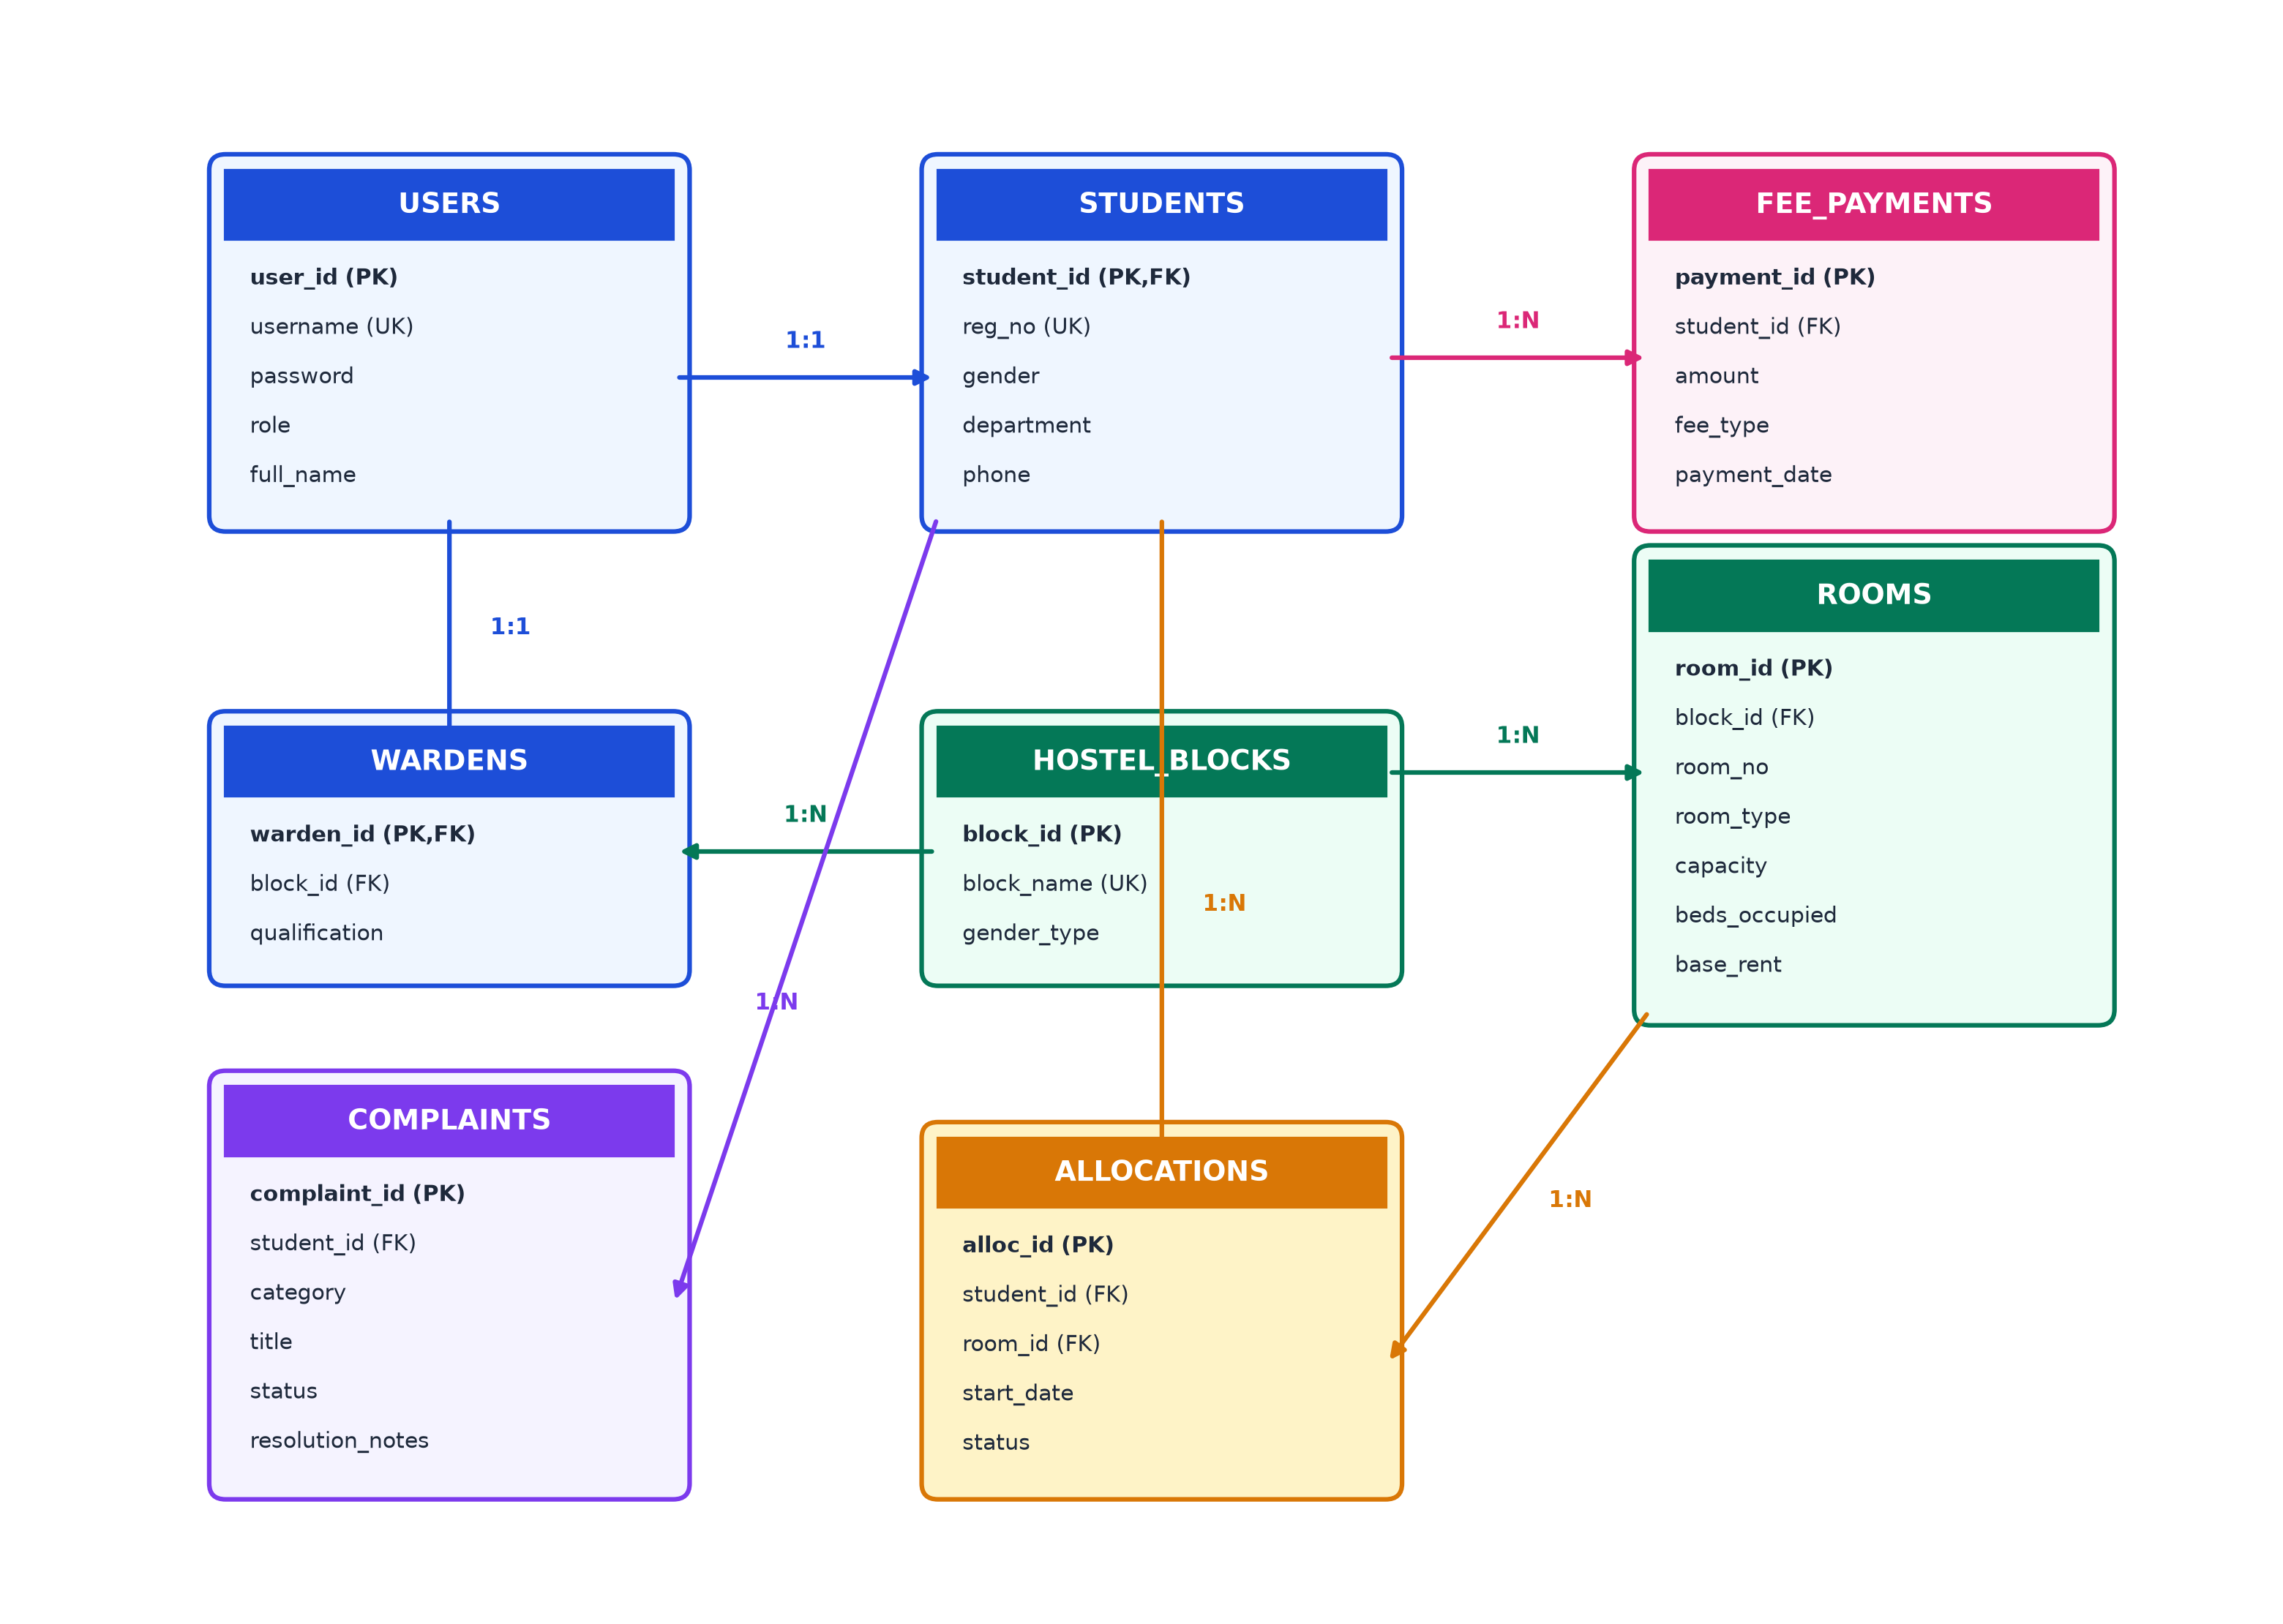
\includegraphics[width=0.95\textwidth]{diagrams/fig3_2_er_diagram.png}
\caption{Entity-Relationship (ER) Crow\'s Foot Schema Diagram}
\label{fig:er_diagram}
\end{figure}


\section{UML Class Hierarchy Design}
The object-oriented domain layer models these entities through two inheritance hierarchies:
\begin{enumerate}
\item \textbf{User Taxonomy:} A base class \texttt{User} defines shared attributes (\texttt{userId}, \texttt{username}, \texttt{password}, \texttt{role}, \texttt{fullName}). The \texttt{Student} subclass extends \texttt{User}, adding university-specific fields (\texttt{regNo}, \texttt{gender}, \texttt{department}, \texttt{phone}).
\item \textbf{Room Taxonomy:} An abstract base class \texttt{Room} defines general room properties (\texttt{roomId}, \texttt{roomNo}, \texttt{capacity}, \texttt{bedsOccupied}, \texttt{baseRent}) and declares an abstract method \texttt{calculateRent()}. Concrete subclasses (\texttt{StandardRoom}, \texttt{DeluxeRoom}, \texttt{ACRoom}) override this method to compute specialized tariffs.
\end{enumerate}

\begin{figure}[htbp]
\centering
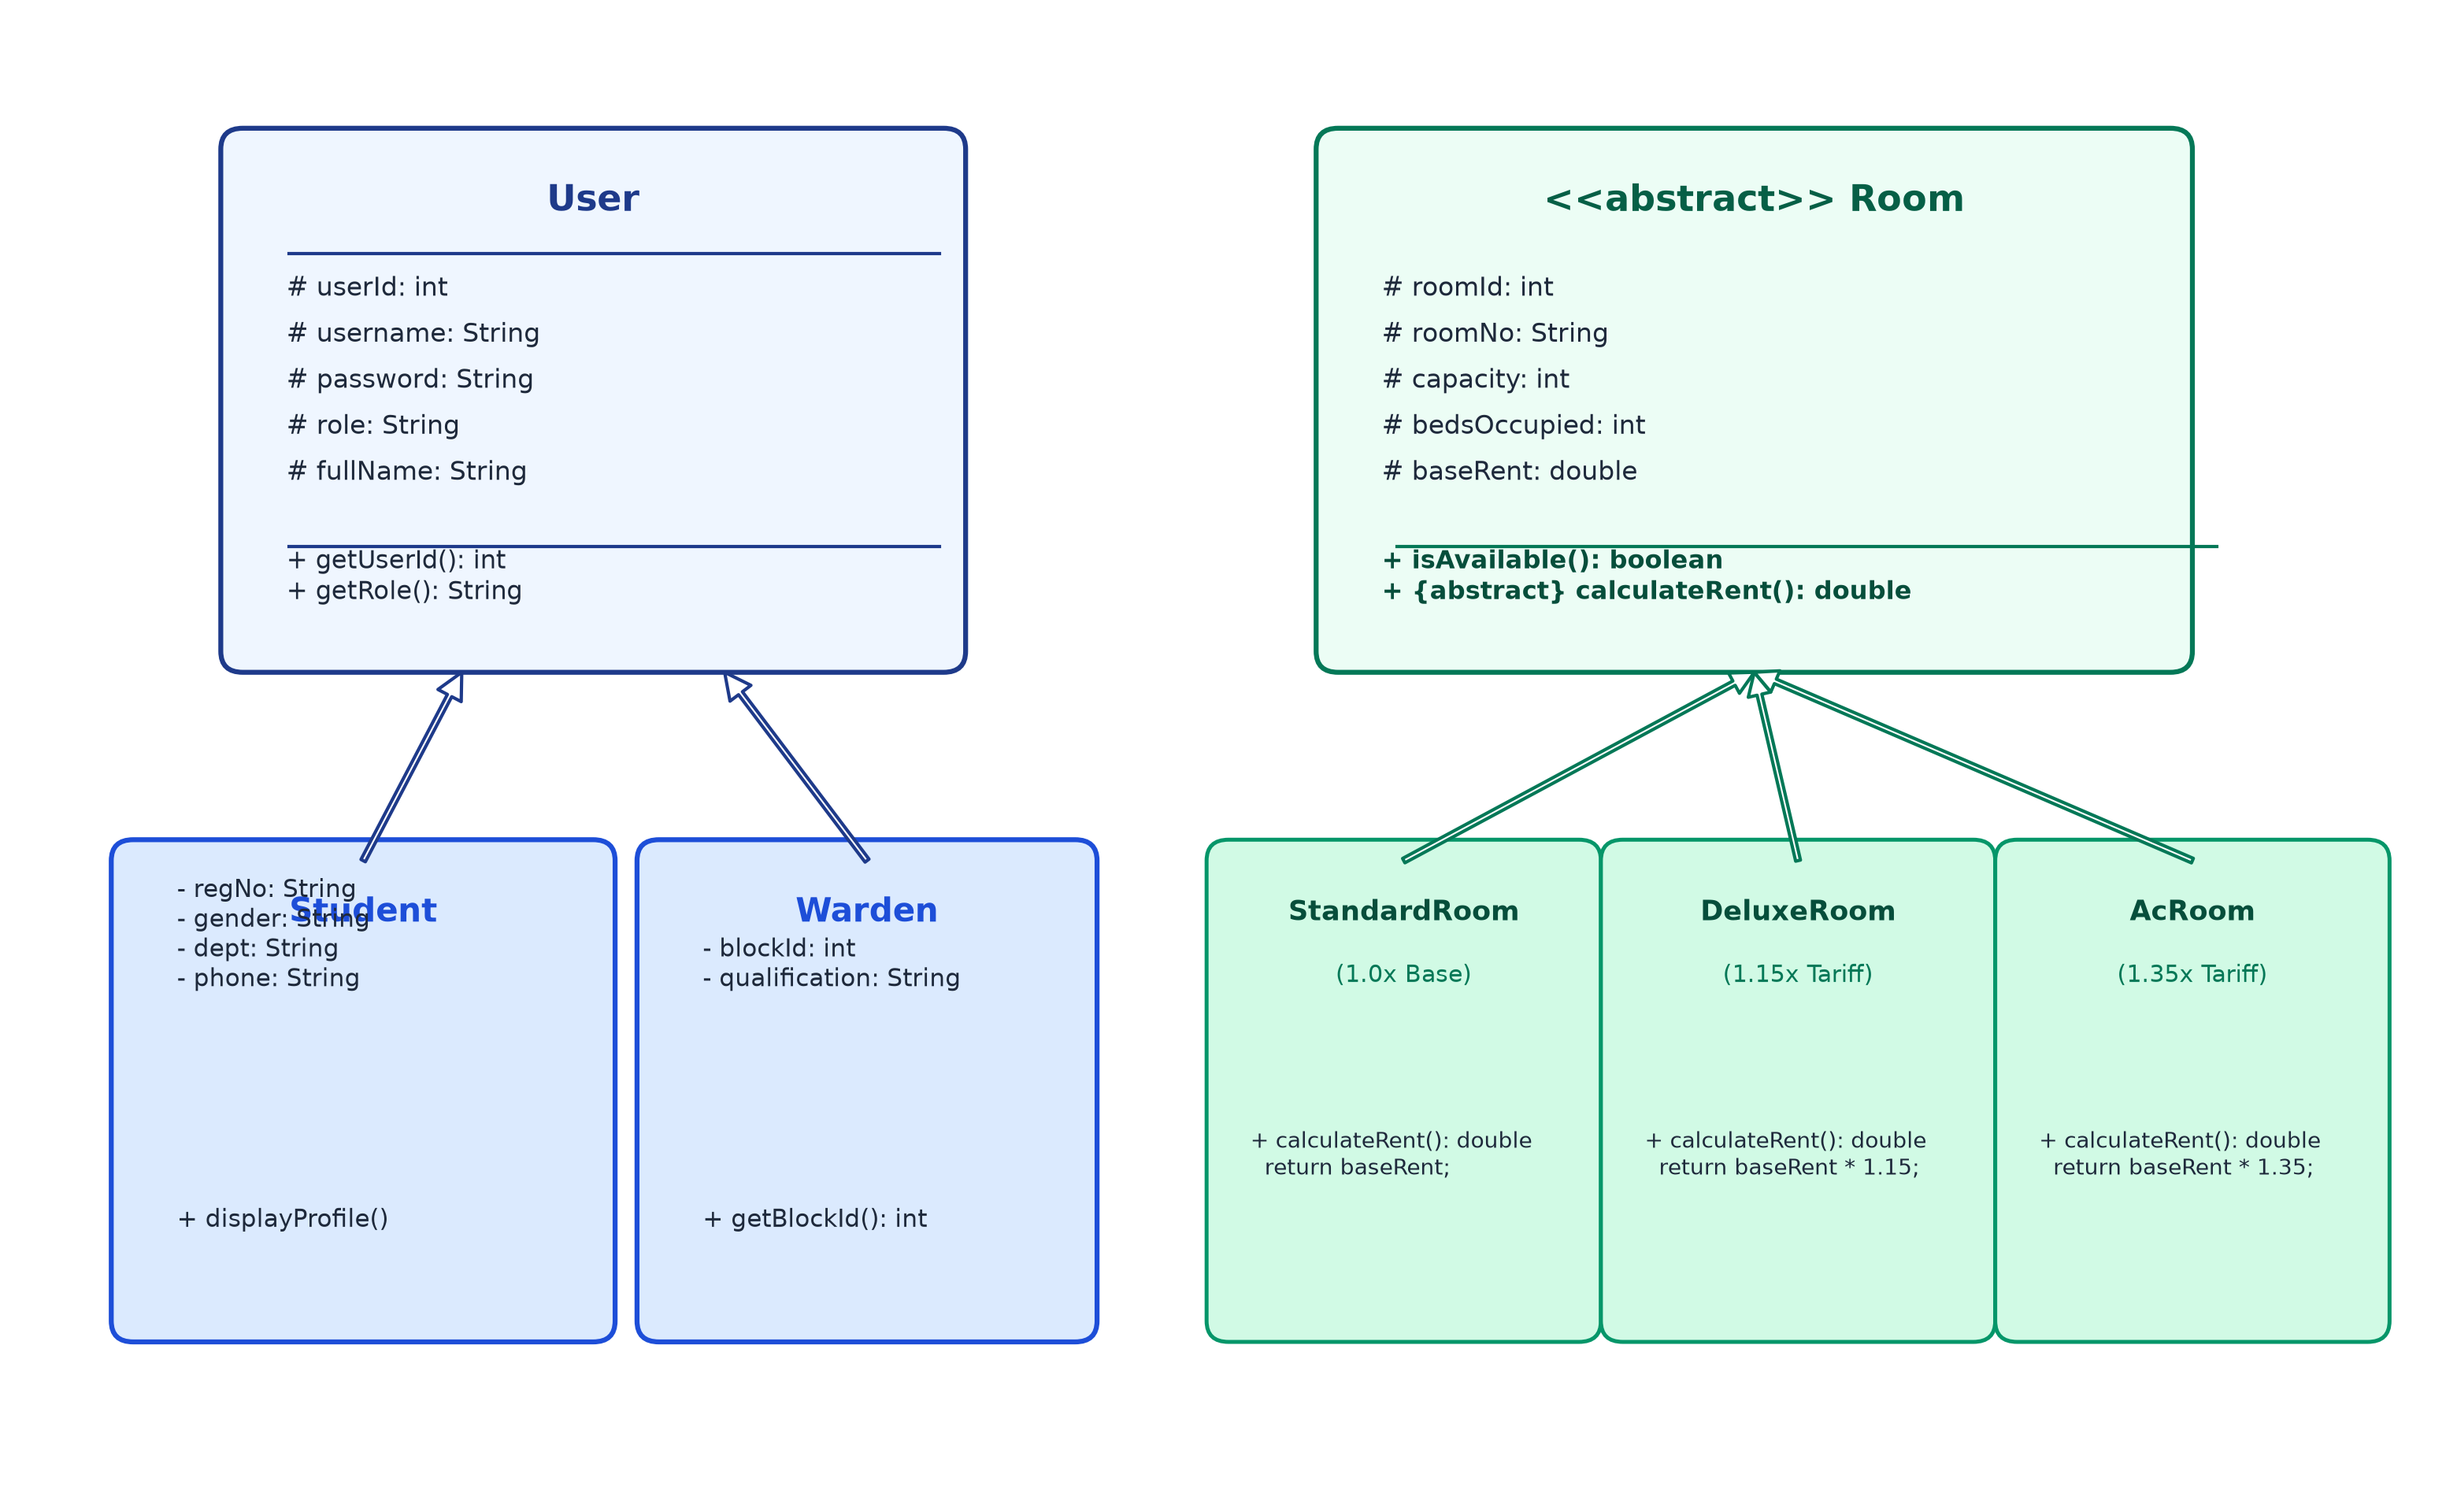
\includegraphics[width=0.95\textwidth]{diagrams/fig3_3_uml_diagram.png}
\caption{UML Object-Oriented Domain Class Diagram}
\label{fig:uml_diagram}
\end{figure}


\section{Mathematical Functional Dependency Analysis and Normalization Proofs}
To provide a rigorous theoretical foundation, the eight relations are analyzed using formal functional dependency (FD) theory:
\begin{itemize}
\item \textbf{Relation 1: USERS ($U$)}
\begin{align*}
U &= (\text{user\_id}, \text{username}, \text{password}, \text{role}, \text{full\_name}) \\
F_U &= \{ \text{user\_id} \to \{\text{username}, \text{password}, \text{role}, \text{full\_name}\}, \; \text{username} \to \{\text{user\_id}, \text{password}, \text{role}, \text{full\_name}\} \}
\end{align*}
Candidate Keys: $\{\text{user\_id}\}$, $\{\text{username}\}$. Since every determinant is a superkey, $U$ satisfies Boyce-Codd Normal Form (BCNF).

\item \textbf{Relation 2: STUDENTS ($S$)}
\begin{align*}
S &= (\text{student\_id}, \text{reg\_no}, \text{gender}, \text{department}, \text{phone}) \\
F_S &= \{ \text{student\_id} \to \{\text{reg\_no}, \text{gender}, \text{department}, \text{phone}\}, \; \text{reg\_no} \to \{\text{student\_id}, \text{gender}, \text{department}, \text{phone}\} \}
\end{align*}
Candidate Keys: $\{\text{student\_id}\}$, $\{\text{reg\_no}\}$. Every determinant is a candidate key; thus, $S$ satisfies BCNF.

\item \textbf{Relation 3: HOSTEL\_BLOCKS ($B$)}
\begin{align*}
B &= (\text{block\_id}, \text{block\_name}, \text{gender\_type}) \\
F_B &= \{ \text{block\_id} \to \{\text{block\_name}, \text{gender\_type}\}, \; \text{block\_name} \to \{\text{block\_id}, \text{gender\_type}\} \}
\end{align*}
Candidate Keys: $\{\text{block\_id}\}$, $\{\text{block\_name}\}$. Meets BCNF.

\item \textbf{Relation 4: ROOMS ($R$)}
\begin{align*}
R &= (\text{room\_id}, \text{block\_id}, \text{room\_no}, \text{room\_type}, \text{capacity}, \text{beds\_occupied}, \text{base\_rent}) \\
F_R &= \{ \text{room\_id} \to \{\text{block\_id}, \text{room\_no}, \text{room\_type}, \text{capacity}, \text{beds\_occupied}, \text{base\_rent}\}, \\
&\quad\; (\text{block\_id}, \text{room\_no}) \to \{\text{room\_id}, \text{room\_type}, \text{capacity}, \text{beds\_occupied}, \text{base\_rent}\} \}
\end{align*}
Candidate Keys: $\{\text{room\_id}\}$, $\{(\text{block\_id}, \text{room\_no})\}$. Notice that room rent and capacity depend on the room record itself rather than the block, avoiding transitive dependencies. Relation satisfies BCNF.

\item \textbf{Relation 6: ALLOCATIONS ($A$)}
\begin{align*}
A &= (\text{alloc\_id}, \text{student\_id}, \text{room\_id}, \text{start\_date}, \text{status}) \\
F_A &= \{ \text{alloc\_id} \to \{\text{student\_id}, \text{room\_id}, \text{start\_date}, \text{status}\} \}
\end{align*}
Candidate Key: $\{\text{alloc\_id}\}$. Resolves the many-to-many relationship between students and rooms across time. Relation satisfies BCNF.
\end{itemize}

\section{Relational Integrity Constraints and DDL Implementation}
The physical relational schema enforces referential actions and domain validation at the database engine level:
\begin{lstlisting}[language=SQL, caption={Core Schema DDL with Referential and Check Constraints}]
-- Enforce foreign key constraints in SQLite
PRAGMA foreign_keys = ON;

CREATE TABLE rooms (
    room_id INTEGER PRIMARY KEY AUTOINCREMENT,
    block_id INTEGER NOT NULL REFERENCES hostel_blocks(block_id) ON DELETE RESTRICT,
    room_no TEXT NOT NULL,
    room_type TEXT NOT NULL CHECK(room_type IN ('STANDARD', 'DELUXE', 'AC')),
    capacity INTEGER NOT NULL CHECK(capacity > 0),
    beds_occupied INTEGER NOT NULL DEFAULT 0 CHECK(beds_occupied >= 0 AND beds_occupied <= capacity),
    base_rent REAL NOT NULL CHECK(base_rent >= 0.0),
    UNIQUE(block_id, room_no)
);

CREATE TABLE allocations (
    alloc_id INTEGER PRIMARY KEY AUTOINCREMENT,
    student_id INTEGER NOT NULL REFERENCES students(student_id) ON DELETE RESTRICT,
    room_id INTEGER NOT NULL REFERENCES rooms(room_id) ON DELETE RESTRICT,
    start_date TEXT NOT NULL DEFAULT (date('now')),
    status TEXT NOT NULL DEFAULT 'ACTIVE' CHECK(status IN ('ACTIVE', 'VACATED'))
);
\end{lstlisting}

\section{System Architecture}
The software follows an enterprise three-tier architecture:
\begin{itemize}
\item \textbf{Presentation Tier:} Delivers two user interfaces sharing identical business logic: a terminal-based Command-Line Interface (\texttt{Main.java}) and an embedded HTTP web dashboard (\texttt{index.html}).
\item \textbf{Application Logic Tier:} Comprises four functional modules (\texttt{StudentModule}, \texttt{RoomModule}, \texttt{AllocationModule}, \texttt{BillingAndComplaintModule}) encapsulating domain rules and transactions.
\item \textbf{Data Persistence Tier:} A centralized database connection pool (\texttt{Database.java}) executing parameterized SQL statements against the normalized relational database.
\end{itemize}

\begin{figure}[htbp]
\centering
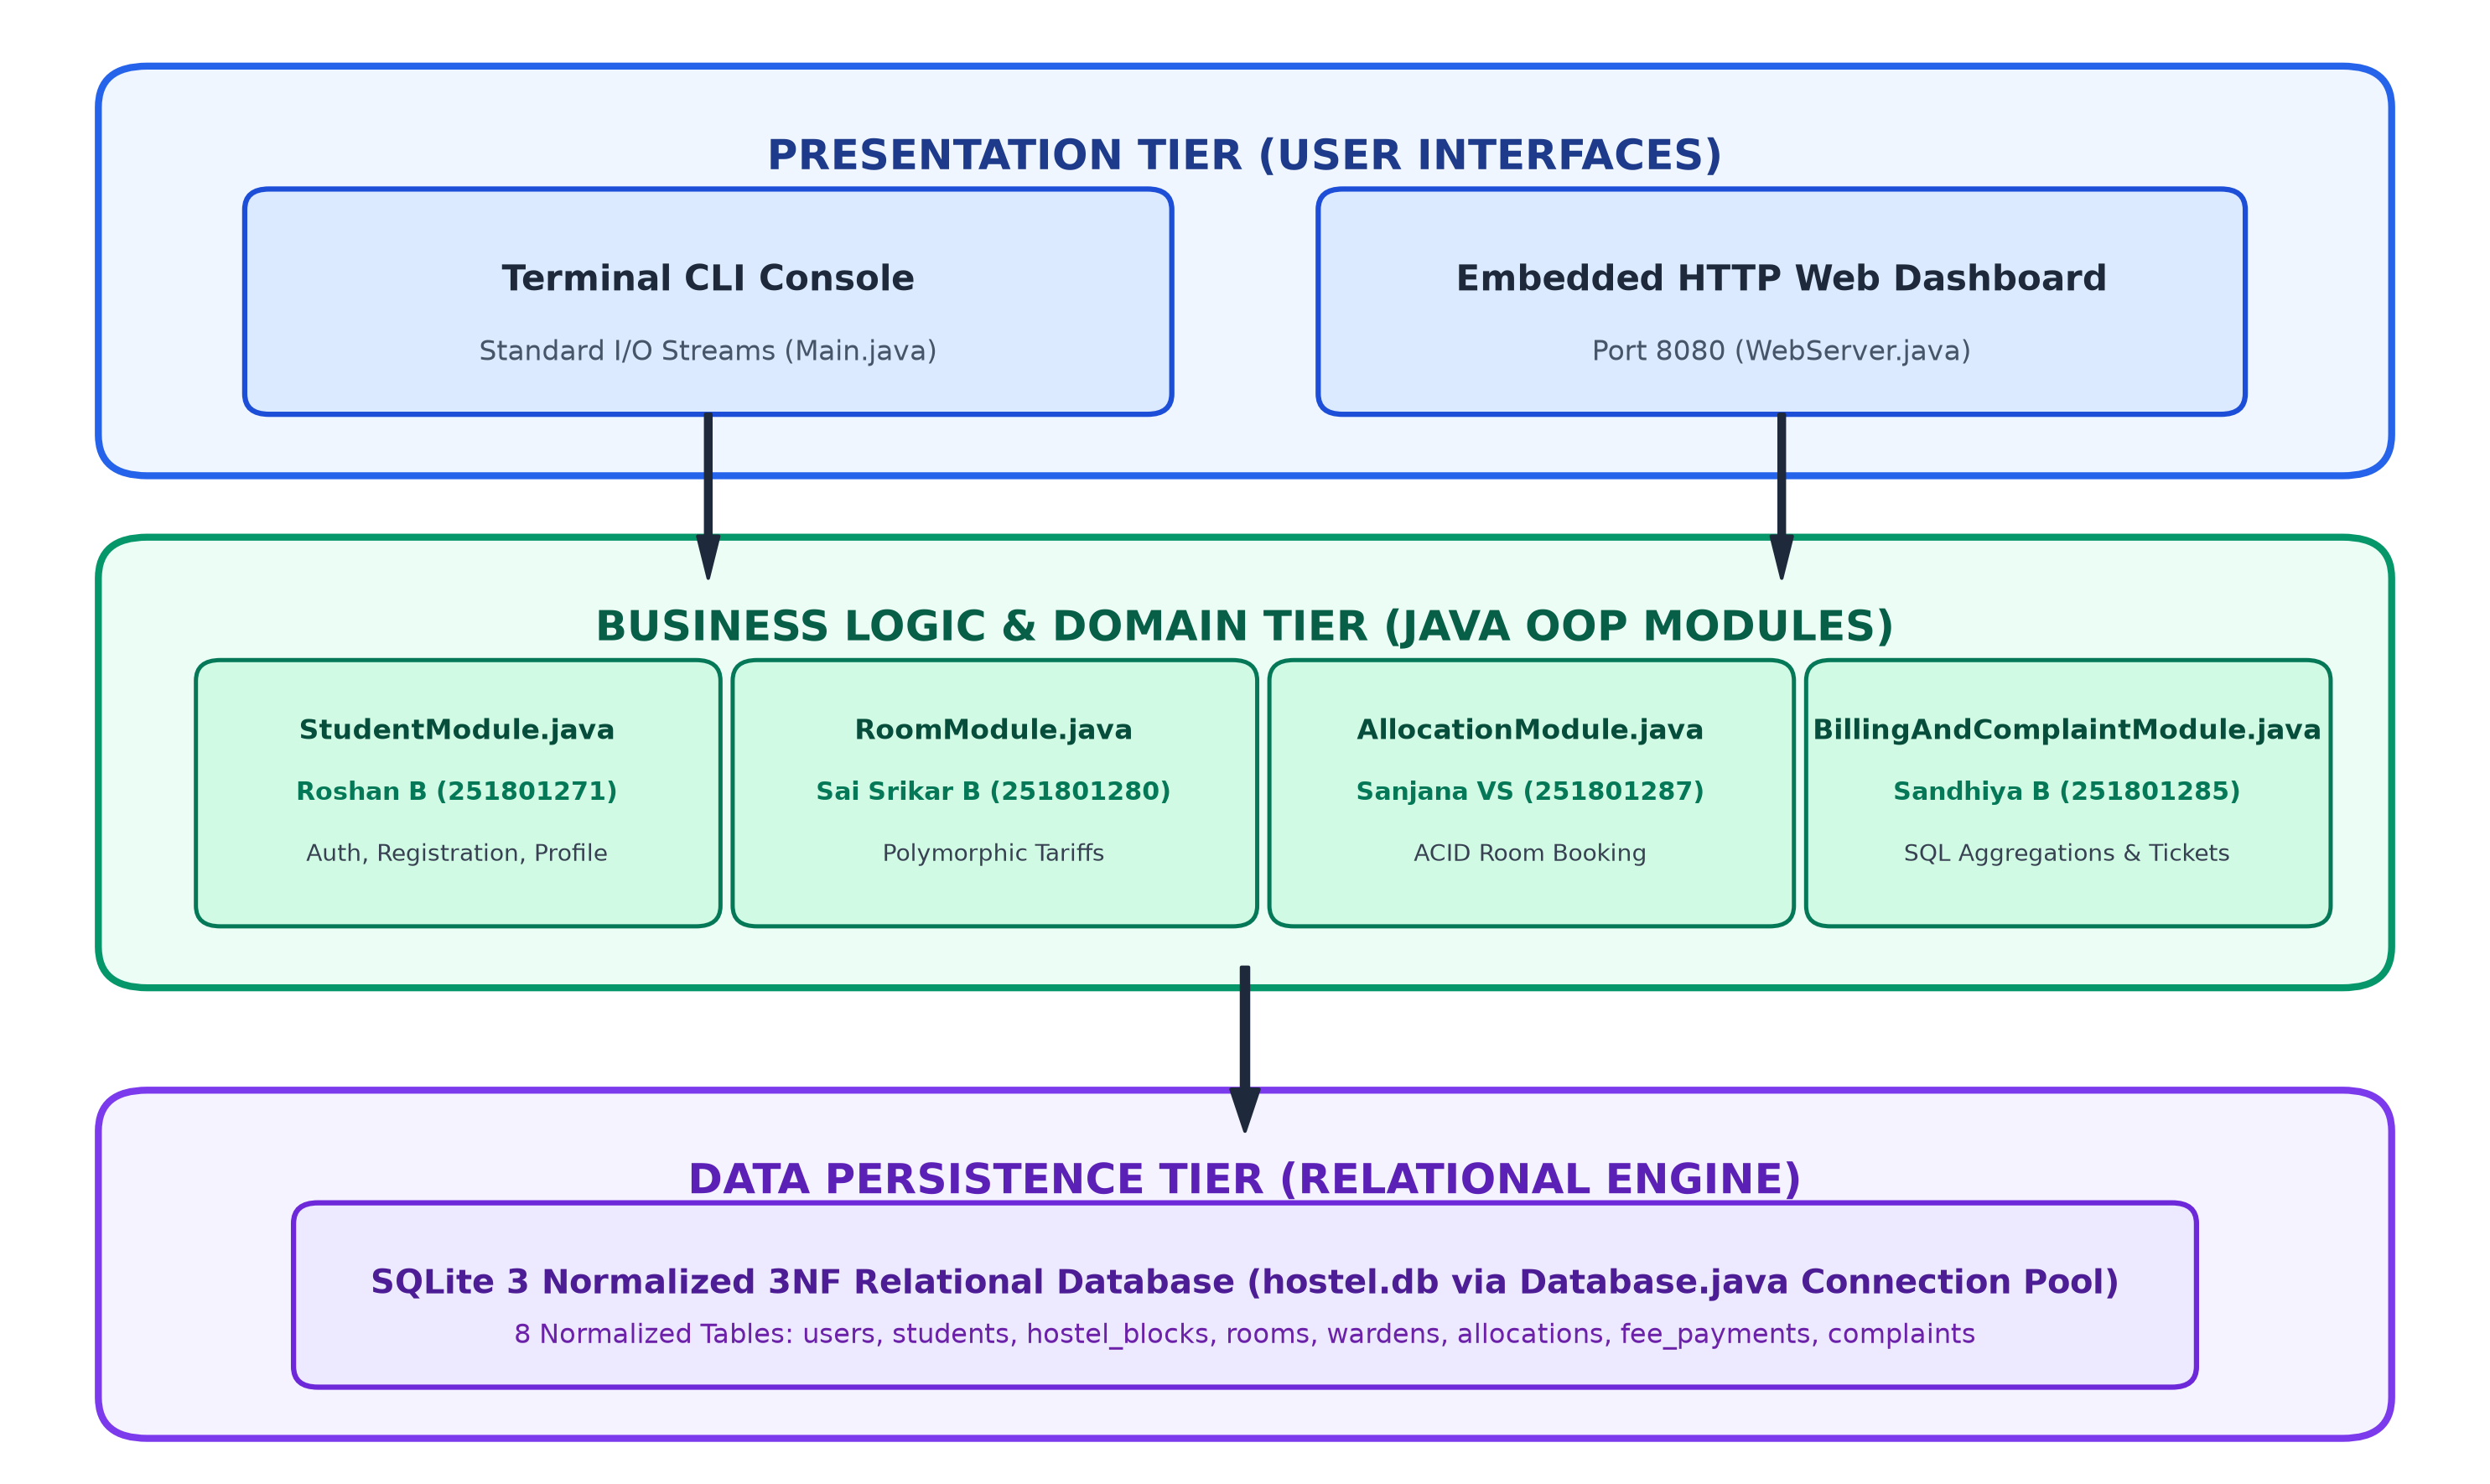
\includegraphics[width=0.95\textwidth]{diagrams/fig3_1_architecture.png}
\caption{Three-Tier Modular System Architecture Flow}
\label{fig:architecture}
\end{figure}


\section{Hardware and Software Specifications}

\begin{table}[h]
\centering
\caption{System Specifications}
\begin{tabular}{ll}
\toprule
\textbf{Component} & \textbf{Specification} \\
\midrule
Processor & Dual Core x86/x64, 2.0 GHz or higher \\
System Memory (RAM) & 4 GB DDR4 minimum (8 GB recommended) \\
Storage & 256 GB Solid State Drive (SSD) \\
Operating System & Microsoft Windows 10/11, Ubuntu Linux, or macOS \\
Programming Language & Java (JDK 17 or JDK 25) \\
Database Engine & Embedded SQLite 3.45 / MySQL Connector/J 9.7 \\
Web Server & Standard Library \texttt{com.sun.net.httpserver.HttpServer} \\
Frontend Technologies & HTML5, CSS3, Vanilla JavaScript \\
Development Environment & IntelliJ IDEA / Visual Studio Code / Terminal \\
\bottomrule
\end{tabular}
\end{table}

\newpage

% CHAPTER 4
\chapter{METHODOLOGY}

\section{Module 1: User Identity and Student Enrollment}
\textbf{Developer:} Roshan B (Register Number: 251801271)\\
\textbf{Assigned Tables:} \texttt{users} (Table 1) and \texttt{students} (Table 2)

\subsection{Object-Oriented Design}
The module demonstrates inheritance and encapsulation. The \texttt{User} base class stores system-wide credentials:
\begin{lstlisting}[language=Java]
class User {
    private int userId;
    private String username;
    private String password;
    private String role;
    private String fullName;

    public User(int userId, String username, String password, 
                String role, String fullName) {
        this.userId = userId;
        this.username = username;
        this.password = password;
        this.role = role;
        this.fullName = fullName;
    }
    public int getUserId() { return userId; }
    public String getUsername() { return username; }
    public String getRole() { return role; }
    public String getFullName() { return fullName; }
}
\end{lstlisting}

The derived \texttt{Student} class inherits from \texttt{User}, adding university attributes:
\begin{lstlisting}[language=Java]
class Student extends User {
    private String regNo;
    private String gender;
    private String department;
    private String phone;

    public Student(int userId, String username, String password, 
                   String fullName, String regNo, String gender, 
                   String department, String phone) {
        super(userId, username, password, "STUDENT", fullName);
        this.regNo = regNo;
        this.gender = gender;
        this.department = department;
        this.phone = phone;
    }
    public String getRegNo() { return regNo; }
    public String getGender() { return gender; }
    public String getDepartment() { return department; }
    public String getPhone() { return phone; }
}
\end{lstlisting}

\subsection{Database Integration}
Student enrollment inserts records into both \texttt{users} and \texttt{students} tables within an explicit transaction:
\begin{lstlisting}[language=Java]
conn.setAutoCommit(false);
try (PreparedStatement ps1 = conn.prepareStatement(userSql, 
        Statement.RETURN_GENERATED_KEYS)) {
    ps1.setString(1, username);
    ps1.setString(2, password);
    ps1.setString(3, fullName);
    ps1.executeUpdate();
    var keys = ps1.getGeneratedKeys();
    keys.next();
    int newUserId = keys.getInt(1);

    try (PreparedStatement ps2 = conn.prepareStatement(studentSql)) {
        ps2.setInt(1, newUserId);
        ps2.setString(2, regNo);
        ps2.setString(3, gender);
        ps2.setString(4, dept);
        ps2.setString(5, phone);
        ps2.executeUpdate();
    }
    conn.commit();
} catch (SQLException e) {
    conn.rollback();
}
\end{lstlisting}

\section{Module 2: Infrastructure Inventory and Polymorphic Tariffs}
\textbf{Developer:} Sai Srikar B (Register Number: 251801280)\\
\textbf{Assigned Tables:} \texttt{hostel\_blocks} (Table 3) and \texttt{rooms} (Table 4)

\subsection{Object-Oriented Design}
The module demonstrates abstraction and polymorphism. An abstract class \texttt{Room} declares an abstract tariff method:
\begin{lstlisting}[language=Java]
abstract class Room {
    private int roomId;
    private int blockId;
    private String roomNo;
    private String roomType;
    private int capacity;
    private int bedsOccupied;
    private double baseRent;

    public abstract double calculateRent(); // Polymorphic method
}
\end{lstlisting}

Concrete subclasses override \texttt{calculateRent()} to calculate specialized pricing:
\begin{lstlisting}[language=Java]
class StandardRoom extends Room {
    public StandardRoom(int id, int bId, String no, int cap, 
                        int occ, double rent) {
        super(id, bId, no, "STANDARD", cap, occ, rent);
    }
    @Override
    public double calculateRent() {
        return getBaseRent(); // Standard base rate
    }
}

class DeluxeRoom extends Room {
    public DeluxeRoom(int id, int bId, String no, int cap, 
                      int occ, double rent) {
        super(id, bId, no, "DELUXE", cap, occ, rent);
    }
    @Override
    public double calculateRent() {
        return getBaseRent() * 1.15; // 15% deluxe amenity surcharge
    }
}

class ACRoom extends Room {
    public ACRoom(int id, int bId, String no, int cap, 
                  int occ, double rent) {
        super(id, bId, no, "AC", cap, occ, rent);
    }
    @Override
    public double calculateRent() {
        return getBaseRent() * 1.35; // 35% HVAC cooling tariff
    }
}
\end{lstlisting}

\subsection{Compile-Time Polymorphism (Method Overloading)}
The module implements method overloading by defining two search methods with differing parameter types:
\begin{lstlisting}[language=Java]
// Overloaded search 1: by minimum bed capacity
public void searchRooms(int minCapacity) {
    String sql = "SELECT * FROM rooms WHERE capacity >= ?";
    searchQuery(sql, minCapacity, null);
}

// Overloaded search 2: by room type
public void searchRooms(String roomType) {
    String sql = "SELECT * FROM rooms WHERE UPPER(room_type) = UPPER(?)";
    searchQuery(sql, null, roomType);
}
\end{lstlisting}

\section{Module 3: Staff Operations and ACID Room Allocations}
\textbf{Developer:} Sanjana VS (Register Number: 251801287)\\
\textbf{Assigned Tables:} \texttt{wardens} (Table 5) and \texttt{allocations} (Table 6)

\begin{figure}[htbp]
\centering
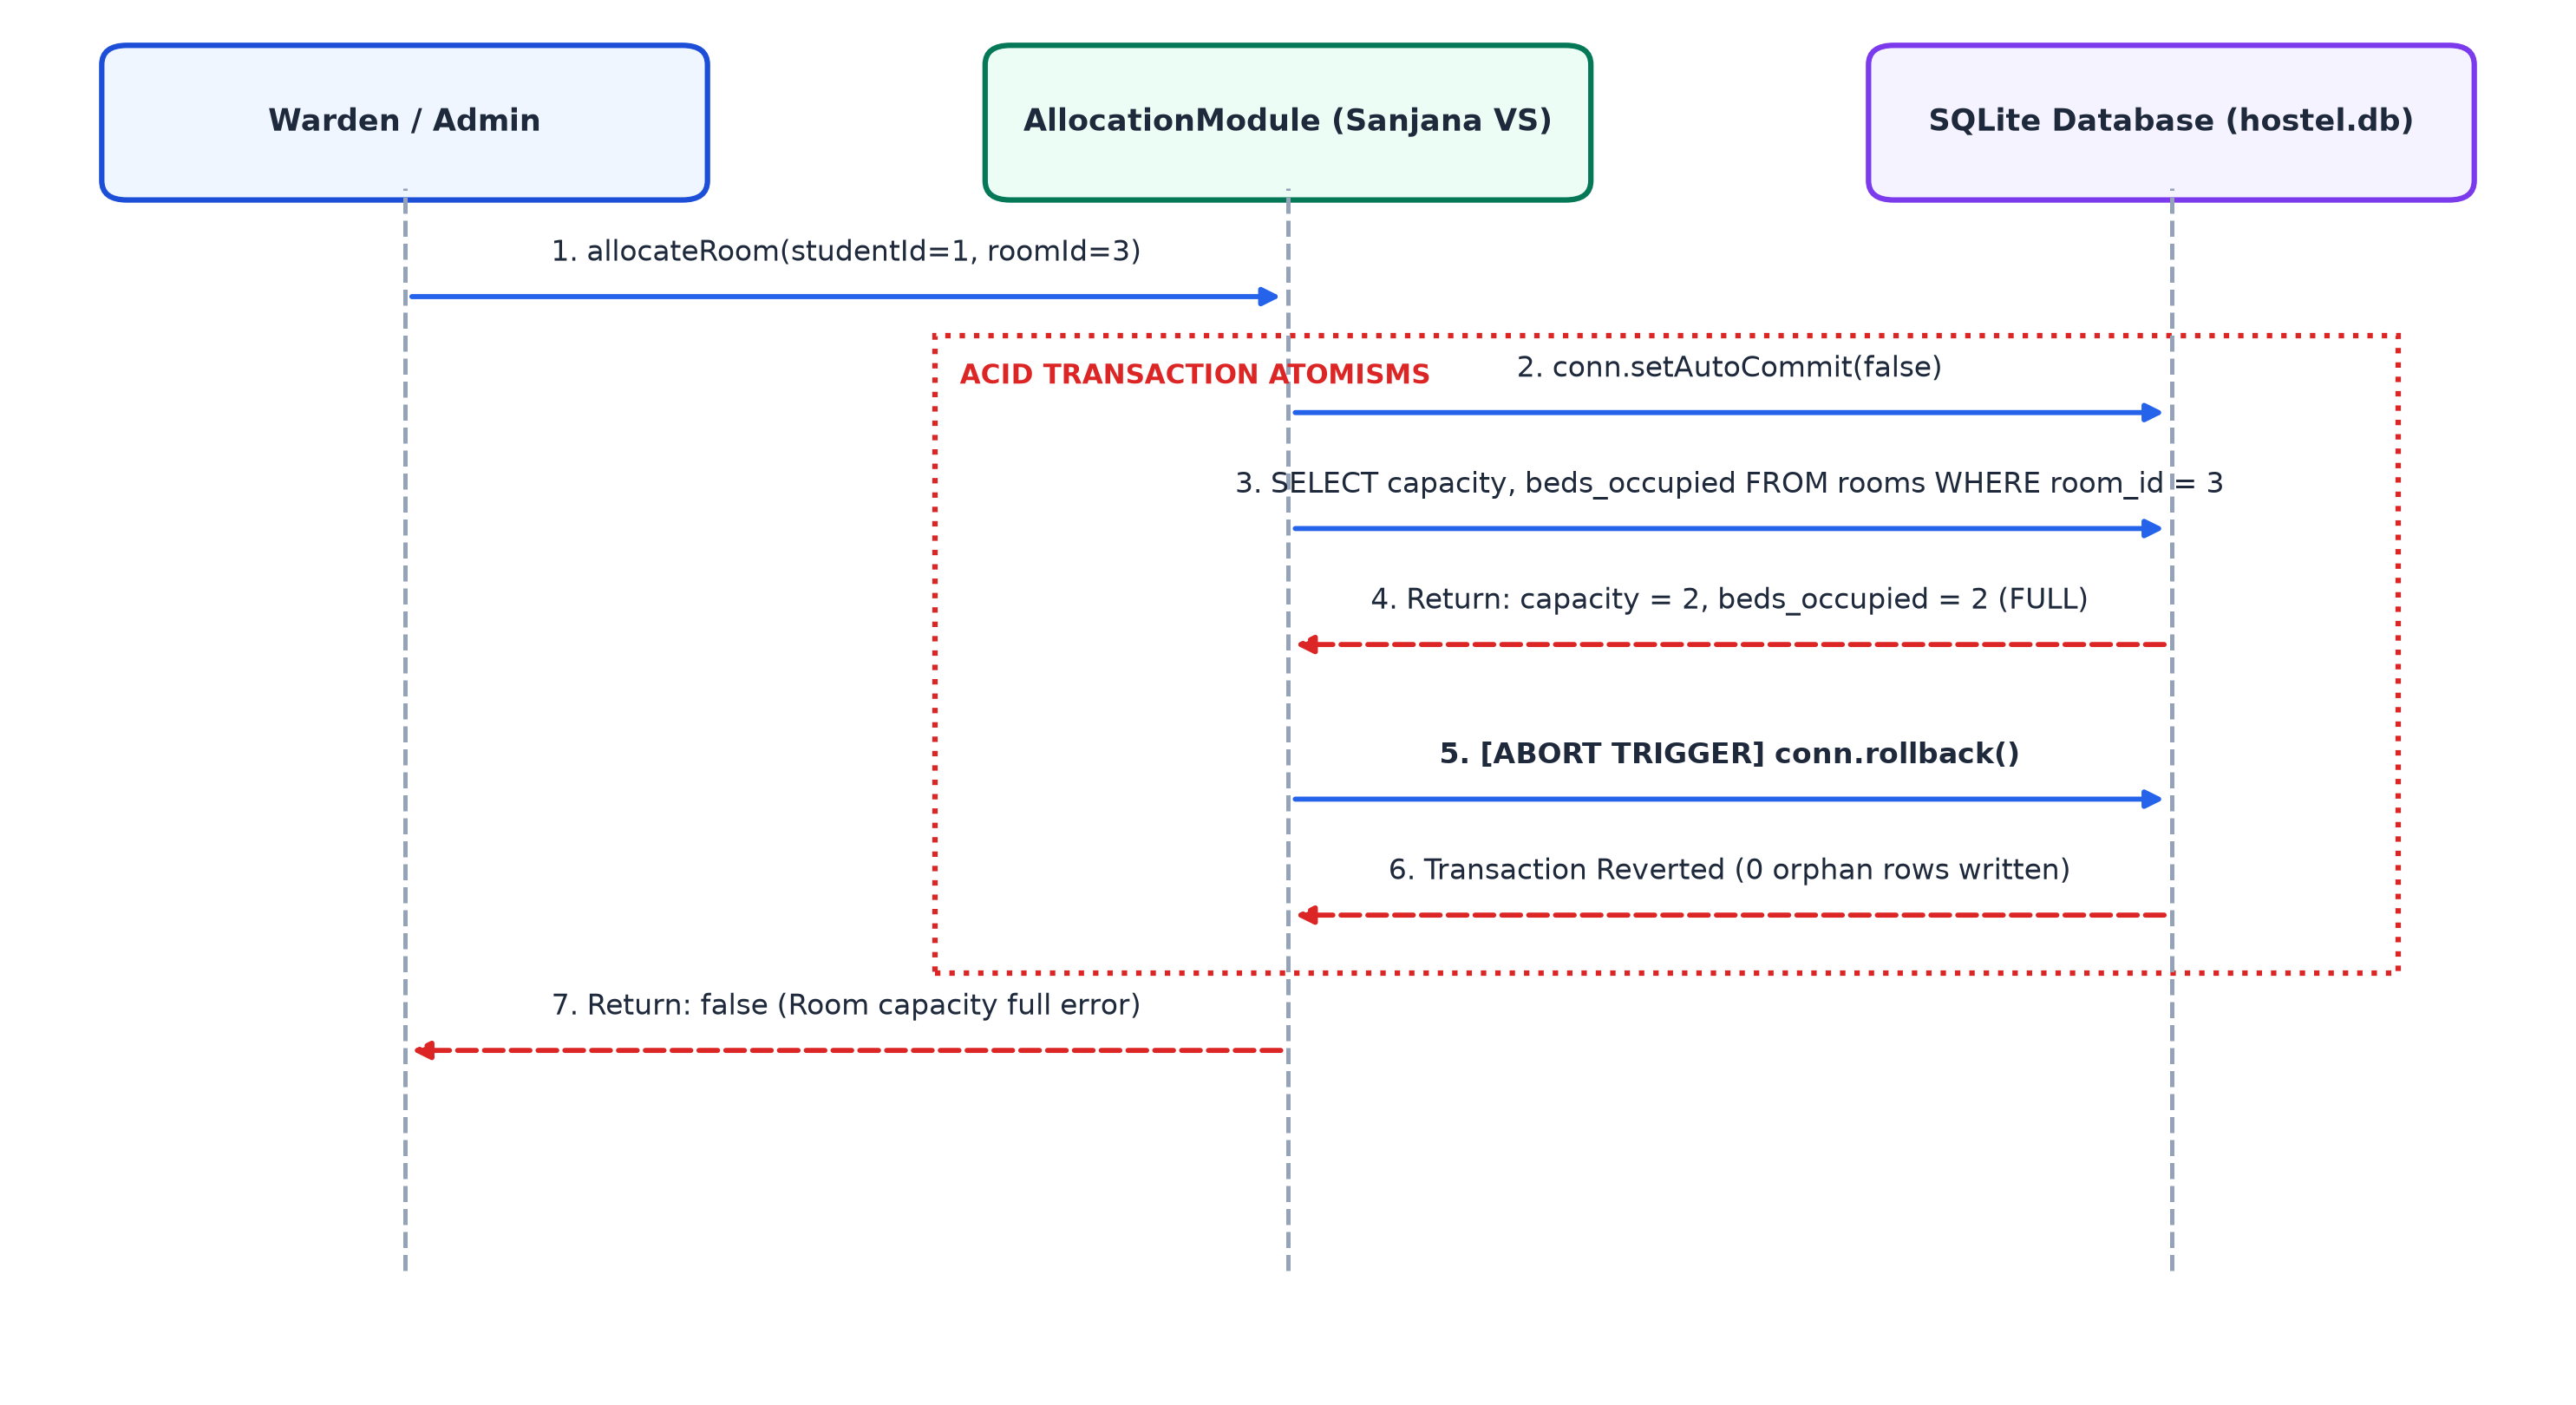
\includegraphics[width=0.95\textwidth]{diagrams/fig4_1_sequence_diagram.png}
\caption{ACID Allocation Transaction Sequence Diagram}
\label{fig:sequence_diagram}
\end{figure}


\subsection{ACID Transaction Implementation}
Assigning a student to a room requires updating two tables atomically. The transaction steps are:
\begin{enumerate}
\item \textbf{Start Transaction:} Disable automatic committing via \texttt{conn.setAutoCommit(false)}.
\item \textbf{Eligibility Validation:} Check that the student does not hold an existing \texttt{ACTIVE} allocation:
\begin{lstlisting}[language=SQL]
SELECT COUNT(*) FROM allocations WHERE student_id = ? AND status = 'ACTIVE';
\end{lstlisting}
\item \textbf{Capacity Validation:} Verify that the room has at least one vacant bed:
\begin{lstlisting}[language=SQL]
SELECT capacity, beds_occupied FROM rooms WHERE room_id = ?;
\end{lstlisting}
If \texttt{beds\_occupied} $\ge$ \texttt{capacity}, invoke \texttt{conn.rollback()} and exit.
\item \textbf{Insert Allocation:} Insert a new row into the \texttt{allocations} table:
\begin{lstlisting}[language=SQL]
INSERT INTO allocations (student_id, room_id, start_date, status) 
VALUES (?, ?, '2026-07-01', 'ACTIVE');
\end{lstlisting}
\item \textbf{Increment Bed Counter:} Increment \texttt{beds\_occupied} in the \texttt{rooms} table:
\begin{lstlisting}[language=SQL]
UPDATE rooms SET beds_occupied = beds_occupied + 1 WHERE room_id = ?;
\end{lstlisting}
\item \textbf{Commit:} Persist changes atomically via \texttt{conn.commit()}. On any SQL exception, execute \texttt{conn.rollback()}.
\end{enumerate}

\section{Module 4: Fee Billing and Grievance Management}
\textbf{Developer:} Sandhiya B (Register Number: 251801285)\\
\textbf{Assigned Tables:} \texttt{fee\_payments} (Table 7) and \texttt{complaints} (Table 8)

\begin{figure}[htbp]
\centering
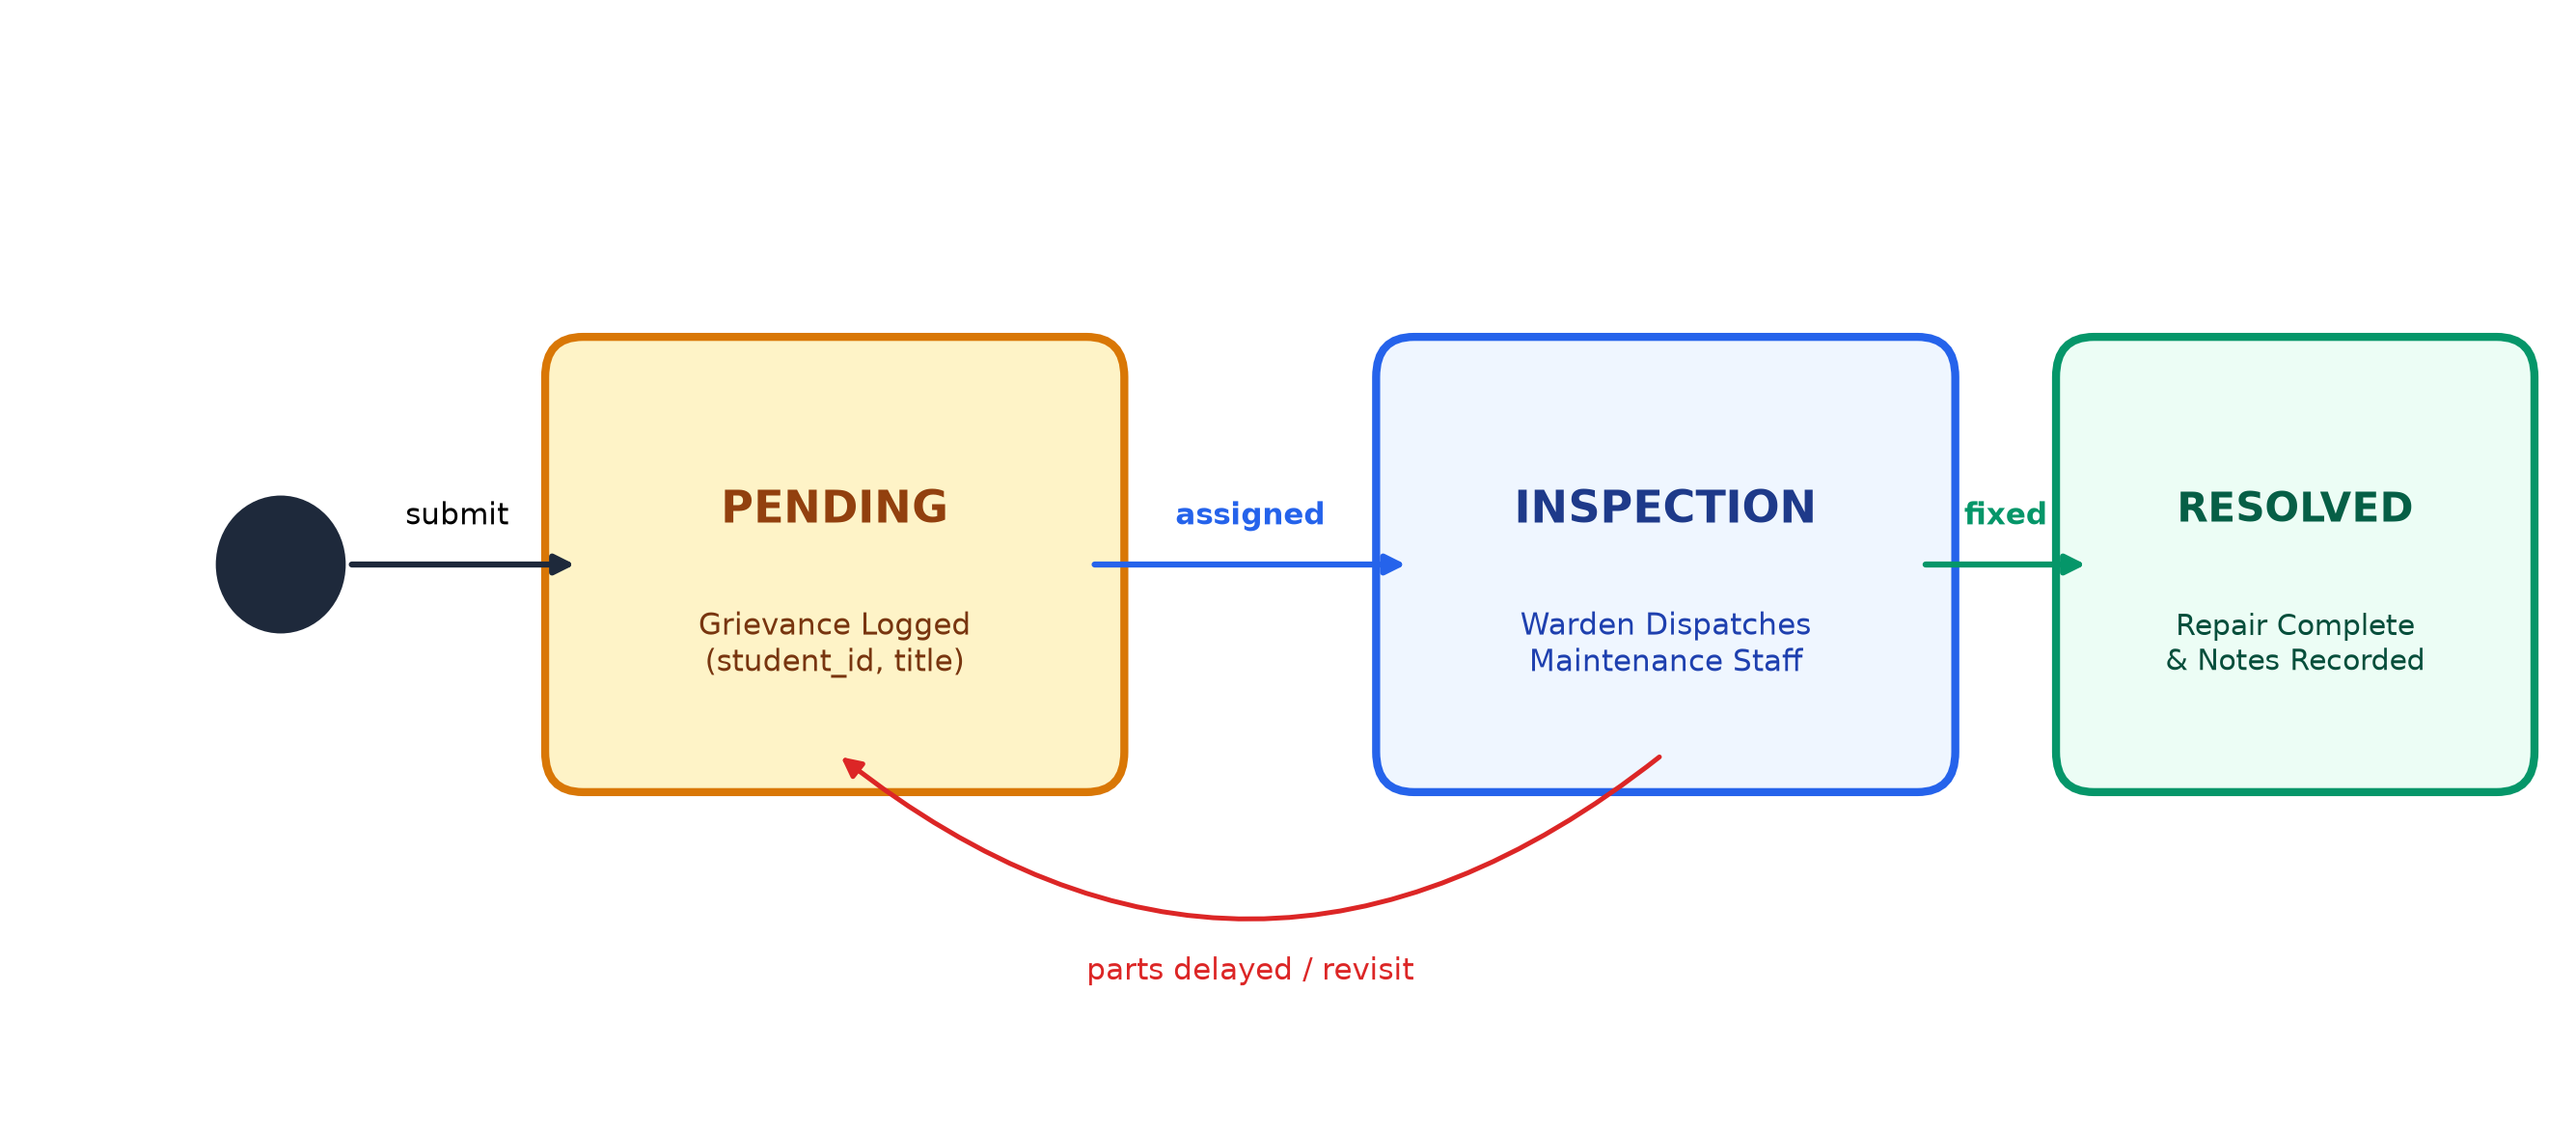
\includegraphics[width=0.85\textwidth]{diagrams/fig4_2_state_machine.png}
\caption{Grievance Lifecycle Finite State Transition Diagram}
\label{fig:state_machine}
\end{figure}


\subsection{Polymorphic Rate Integration}
Rather than hardcoding room rates in the billing module, the semester bill is computed by querying the resident's allocated room and invoking Member 2's polymorphic method:
\begin{lstlisting}[language=Java]
public double calculateTotalSemesterBill(int studentId) {
    String sql = "SELECT r.* FROM rooms r JOIN allocations a " +
                 "ON r.room_id = a.room_id " +
                 "WHERE a.student_id = ? AND a.status = 'ACTIVE'";
    try (PreparedStatement ps = conn.prepareStatement(sql)) {
        ps.setInt(1, studentId);
        ResultSet rs = ps.executeQuery();
        if (rs.next()) {
            Room r = roomModule.createRoomInstance(rs.getInt("room_id"), 
                    rs.getInt("block_id"), rs.getString("room_no"), 
                    rs.getString("room_type"), rs.getInt("capacity"), 
                    rs.getInt("beds_occupied"), rs.getDouble("base_rent"));
            
            // Polymorphic rent calculation * 6 months + mess charges
            return (r.calculateRent() * 6.0) + 15000.0;
        }
    }
    return 0.0;
}
\end{lstlisting}

\subsection{SQL Aggregations}
Total payments made by a resident are calculated via SQL aggregation:
\begin{lstlisting}[language=SQL]
SELECT SUM(amount) AS total FROM fee_payments WHERE student_id = ?;
\end{lstlisting}
The outstanding balance is derived as:
$$\text{Pending Dues} = \max(0,\; \text{Total Semester Bill} - \text{Total Payments Remitted})$$

\section{Database Security and Parameterized Queries}
To protect against SQL injection vulnerabilities, all queries utilize parameterized \texttt{PreparedStatement} objects rather than string concatenation:
\begin{lstlisting}[language=Java]
String sql = "SELECT * FROM users WHERE username = ? AND password = ?";
try (PreparedStatement ps = conn.prepareStatement(sql)) {
    ps.setString(1, inputUser);
    ps.setString(2, inputPass);
    ResultSet rs = ps.executeQuery();
}
\end{lstlisting}
This forces the SQL parser to treat input strictly as parameter literals.

\section{Dual Presentation Interfaces}
The application supports two user interface modes:
\begin{enumerate}
\item \textbf{Terminal Console Interface (\texttt{Main.java}):} Keyboard-driven menus for administrative users operating in command-line environments.
\item \textbf{Embedded HTTP Web Server (\texttt{WebServer.java}):} Uses the built-in \texttt{com.sun.net.httpserver.HttpServer} on port 8080, serving an HTML5/CSS3 Single Page Application connecting through REST endpoints (\texttt{/api/students}, \texttt{/api/rooms}, \texttt{/api/allocations}, \texttt{/api/billing}, \texttt{/api/complaints}).
\end{enumerate}

\newpage

% CHAPTER 5
\chapter{RESULTS AND DISCUSSIONS}

\section{Test Environment Setup}
Testing was conducted on an x64 workstation running OpenJDK 25 and SQLite 3.45. Functional and boundary test cases were evaluated against predefined criteria.

\begin{table}[h]
\centering
\caption{Functional Test Cases and Execution Results}
\resizebox{\textwidth}{!}{
\begin{tabular}{lllll}
\toprule
\textbf{Test ID} & \textbf{Workflow Evaluated} & \textbf{Input Condition} & \textbf{Expected Outcome} & \textbf{Status} \\
\midrule
TC-01 & Student Registration & Complete registration attributes & Records added to \texttt{users} and \texttt{students} & PASS \\
TC-02 & User Authentication & Valid username and password & Authenticated \texttt{User} object returned & PASS \\
TC-03 & Bad Password Handling & Valid username, incorrect password & Returns \texttt{null}, blocks access & PASS \\
TC-04 & Standard Room Tariff & Room base rent: \rupee 4,500 & \texttt{calculateRent()} yields \rupee 4,500.00 & PASS \\
TC-05 & Deluxe Room Tariff & Base rent: \rupee 6,000 (+15\%) & \texttt{calculateRent()} yields \rupee 6,900.00 & PASS \\
TC-06 & AC Room Tariff & Base rent: \rupee 8,500 (+35\%) & \texttt{calculateRent()} yields \rupee 11,475.00 & PASS \\
TC-07 & Over-Allocation Prevention & Booking room where occupied = capacity & Transaction rolled back; bed count unchanged & PASS \\
TC-08 & Duplicate Booking Prevention & Assigning second room to active student & Transaction rolled back with warning & PASS \\
TC-09 & Bed Counter on Vacate & Executing checkout for active resident & Status set to \texttt{VACATED}, beds decremented & PASS \\
TC-10 & Fee Balance Aggregation & Querying balance for billed resident & Computes dues minus payments via \texttt{SUM} & PASS \\
TC-11 & Grievance Ticket Resolution & Warden enters resolution notes on ticket & Status changes from \texttt{PENDING} to \texttt{RESOLVED} & PASS \\
\bottomrule
\end{tabular}
}
\end{table}

\section{Verification of Polymorphic Tariff Calculations}
Executing queries across room subclasses confirmed polymorphic rate calculations:
\begin{itemize}
\item Room K-101 (\texttt{STANDARD}): Base Rent = \rupee 4,500.00 $\to$ Monthly Tariff = \textbf{\rupee 4,500.00}
\item Room K-102 (\texttt{DELUXE}): Base Rent = \rupee 6,000.00 $\to$ Monthly Tariff = \textbf{\rupee 6,900.00} ($6000 \times 1.15$)
\item Room K-103 (\texttt{AC}): Base Rent = \rupee 8,500.00 $\to$ Monthly Tariff = \textbf{\rupee 11,475.00} ($8500 \times 1.35$)
\end{itemize}

\section{ACID Transaction Testing: Concurrency and Rollback}
To verify transactional consistency, two sequential allocation attempts were executed against room K-103 (capacity = 1). The first allocation succeeded, setting \texttt{beds\_occupied} to 1. The second allocation attempt triggered the validation check:
$$\text{beds\_occupied} \ge \text{capacity}$$
The transaction invoked \texttt{conn.rollback()}, ensuring that bed occupancy remained capped at 1.

\section{Fee Ledger and SQL Aggregation Verification}
Billing calculations were tested for resident Rahul Verma (Room K-101):
\begin{itemize}
\item 6 Months Room Rent ($6 \times 4500$): \rupee 27,000.00
\item Semester Catering Fee: \rupee 15,000.00
\item Total Semester Bill: \rupee 42,000.00
\item Remitted Payment: \rupee 27,000.00
\item Outstanding Balance Calculated: \textbf{\rupee 15,000.00} (accurately reflecting unpaid catering charges).
\end{itemize}

\section{Grievance Redressal Verification}
Testing confirmed ticket lifecycle management. Lodging a complaint added a record with \texttt{PENDING} status. When the warden recorded resolution remarks, the record transitioned to \texttt{RESOLVED}, with notes displayed in both terminal and web views.

\newpage

% CHAPTER 6
\chapter{CONCLUSION}

This project presents a verified institutional management system integrating \textbf{Object-Oriented Programming principles} and \textbf{Relational Database Management Systems}. By organizing data into eight normalized tables in Third Normal Form (3NF), the software prevents data redundancy, eliminates room double-booking, and maintains verifiable financial ledgers.

The application reflects clear collaborative division of labor across the four team members:
\begin{itemize}
\item \textbf{Roshan B} constructed the user identity and student enrollment module using inheritance and encapsulation.
\item \textbf{Sai Srikar B} developed the infrastructure inventory and polymorphic tariff calculation engine with method overloading.
\item \textbf{Sanjana VS} implemented atomic multi-table ACID transactions safeguarding room allocations from race conditions.
\item \textbf{Sandhiya B} built fee ledger accounting using SQL aggregations alongside a maintenance ticket state machine.
\end{itemize}

With both a keyboard-driven terminal console and a responsive web dashboard, the system demonstrates that clean, modular code with minimal dependencies can deliver dependable administrative automation.

\newpage

% CHAPTER 7
\chapter{FUTURE ENHANCEMENTS}

\begin{enumerate}
\item \textbf{Biometric and Smart Card Integration:} Connecting physical turnstiles to automatically record student entry and exit timestamps into the database.
\item \textbf{Payment Gateway API Integration:} Connecting digital banking webhooks to automatically verify online fee transactions.
\item \textbf{Automated Notification Dispatchers:} Dispatching automated SMS and email alerts to parents and wardens regarding fee deadlines and gate passes.
\item \textbf{Mobile Application Clients:} Developing companion mobile interfaces in Flutter or React Native communicating with the existing REST backend.
\item \textbf{Audit Logging and Security Trails:} Recording administrative actions in an immutable audit ledger for enhanced accountability.
\end{enumerate}

\newpage

% REFERENCES
\begin{thebibliography}{99}
\bibitem{gosling} J. Gosling, B. Joy, G. Steele, P. Bracha, and A. Buckley, \textit{The Java Language Specification, Java SE 17 Edition}, Addison-Wesley, 2021.
\bibitem{silberschatz} A. Silberschatz, H. F. Korth, and S. Sudarshan, \textit{Database System Concepts}, 7th ed., McGraw-Hill Education, 2019.
\bibitem{elmasri} R. Elmasri and S. B. Navathe, \textit{Fundamentals of Database Systems}, 7th ed., Pearson, 2016.
\bibitem{gamma} E. Gamma, R. Helm, R. Johnson, and J. Vlissides, \textit{Design Patterns: Elements of Reusable Object-Oriented Software}, Addison-Wesley, 1994.
\bibitem{date} C. J. Date, \textit{An Introduction to Database Systems}, 8th ed., Pearson, 2004.
\bibitem{eckel} B. Eckel, \textit{Thinking in Java}, 4th ed., Prentice Hall, 2006.
\bibitem{sqlite} SQLite Development Team, \textit{SQLite Documentation and Architecture Reference}, 2024. [Online]. Available: https://www.sqlite.org/docs.html
\bibitem{jdbc} Oracle Corporation, \textit{Java Database Connectivity (JDBC) API Documentation}, 2023. [Online]. Available: https://docs.oracle.com/javase/8/docs/technotes/guides/jdbc/
\end{thebibliography}

\end{document}
